\documentclass[iop]{emulateapj-rtx4}
%\slugcomment{{\sc Accepted to ApJ:} April 14, 2015}


%\documentclass[12pt]{article}
%\pdfpagewidth 8.5in
%\pdfpageheight 11in 
%\setlength\topmargin{0in}
%\setlength\headheight{0in}
%\setlength\headsep{0in}
%\setlength\textheight{9in}
%\setlength\textwidth{6.5in}
%\setlength\oddsidemargin{0in}
%\setlength\evensidemargin{0in}
\usepackage{graphicx}
\usepackage{amssymb}

%\usepackage{multicol}
%\usepackage{sidecap}
%\usepackage{ragged2e}

%\usepackage{etoolbox}
%\AtBeginEnvironment{multicols}{\RaggedRight}

%\usepackage{epstopdf}
%\usepackage{verbatim}

%\usepackage{caption}
%\usepackage{subcaption}

\usepackage{wrapfig}
\usepackage{setspace}
%\usepackage{subfig}
\usepackage{mathtools}


%\newcommand{\rms}[1]{\langle #1 \rangle}
%\renewcommand{\baselinestretch}{1.5}
%\renewcommand{\thefootnote}{\roman{footnote}}

\graphicspath{{proposal_figures//}}


\frenchspacing

\begin{document}

%\onehalfspacing

\title{Probing the Gaseous Environments of Galaxies}
\author{David M. French \\
Advisor: Dr. Bastiaan Wakker}
%\affil{Proposal for a Ph.D. Thesis: Department of Astronomy, University of Wisconsin - Madison; frenchd@astro.wisc.edu}
\affil{Proposal for a Ph.D. Thesis: Department of Astronomy, University of Wisconsin - Madison}

%\affil{Department of Astronomy, University of Wisconsin - Madison; frenchd@astro.wisc.edu}


\begin{abstract}


Galaxies must accrete gas from the intergalactic medium (IGM) in order to sustain star formation at observed levels. In order to understand this complex process, and how it influences galaxy evolution, it is necessary to understand the physical conditions and distribution of the gas around galaxies, known as the circumgalactic medium (CGM). For my thesis, I propose to use archival spectra of bright background QSOs taken by the Cosmic Origins Spectrograph (COS) on the Hubble Space Telescope (HST) to directly probe the CGM of galaxies in the nearby Universe. I will supplement this spectral data with observations of these galaxies taken by the WIYN and SALT telescopes. This proposed program will be the largest and most statistically significant survey of the local CGM to date.

\end{abstract}
\keywords{IGM, CGM, galaxies}


\section{Galaxy Table:}\\

\subsection{Extinction:}\\

Extinction estimates for galaxies are taken from the Galactic Dust Reddening and Extinction service of IRSA, which provides values derived by Schlegel, Finkbeiner \& Davis (1998) and Schlafly and Finkbeiner (2011) from combined IRAS and COBE/DIRBE results. We use the updated Schlafly \& Finkbeiner 2011 (ApJ 737, 103) values, which are corrections on the original Schlegel et al. 1998 (ApJ 500, 525) values based on the following:

\begin{equation}
E(B-V)_{S~\&~F} = 0.86~*~ E(B-V)_{SFD}
\end{equation}
 
 
 
\section{Introduction}

\indent The majority of the baryons in the universe are found in the diffuse intergalactic medium (IGM). The IGM and the galaxies that reside in it are tightly linked by processes such as feedback and accretion. In order to sustain the levels of star formation observed, galaxies must accrete gas throughout their lifetimes (e.g. see Erb 2008, Putman et al. 2009b). At the same time, ongoing star formation and active galactic nuclei (AGN) activity produce feedback that drives gas back into the IGM. This life cycle of gas is complex, and still poorly constrained. Understanding the properties of the IGM such as its densities, temperatures, and motions, and its relationship to the galaxies embedded within it is \textit{essential} for explaining the evolution of galaxies and the star formation history of the universe. 

\indent The properties of the vast reservoir of material in the IGM can be understood by analyzing lines of sight towards background quasi-stellar objects (QSOs). Individual concentrations of gas along a given sightline imprint a `forest' of absorption lines on the spectrum in the direction of the QSO. The metal lines trace the star formation history within the intervening gas, and neutral hydrogen lines (Ly$\alpha$) indicate both the location and velocities of outflowing gas as well as the presence of fuel for future star formation. The relationship between the galaxies and the IGM is usually studied by looking for galaxies that lie near the redshift of detected absorption lines (see Figure \ref{hubble_cgm} for an illustration). This approach has value, but is incomplete; it does not allow for an unbiased understanding of the distribution of the gas around galaxies, which requires looking for both detections and non-detections of gas, both near as well as far away from galaxies.

\indent The current standard model of structure formation is given by $\Lambda$CDM cosmology, which predicts the hierarchical growth of large scale structures seeded by initial fluctuations in the dark matter background. In this picture, both galaxies and neutral H\,{\sc i} follow the same underlying density profile. Wakker et al. (2015, submitted) have provided some observational evidence for this, showing that Ly$\alpha$ absorption strength traces the large-scale distribution of galaxies in a Cosmic Web filament. In addition, numerous previous studies have shown that Ly$\alpha$ absorbers also trace individual galaxy halos (e.g. Wakker $\&$ Savage 2009, Danforth et al. 2014, Stocke et al. 2013, Liang et al 2014, Lanzetta et al 1995, Chen et al. 1998, 2001a, Tripp et al. 1998, Steidel et al. 2010, Prochaska et al. 2011, Thom et al 2012). 

Recent studies find that about half of Ly$\alpha$ absorbers lie within galaxy haloes, at impact parameters $\rho<350$ kpc (C\^{o}t\'{e} et al. 2005, Prochaska et al. 2006). In addition, Wakker $\&$ Savage (2009) find that for 90$\%$ of L$>0.1L_{\**}$ galaxies an absorber lies within 400 kpc and 400 km/s, and all galaxies have a Ly$\alpha$ absorber within 1.5 Mpc. Higher redshift studies, such as Rudie et al. (2012) at $2<z<3$, find evidence for an elevated density of absorbers up to 2 Mpc from galaxies. Wakker $\&$ Savage (2009) also confirmed a previously suggested correlation between Ly$\alpha$ absorption linewidth ($W$) and impact parameter $\rho$, observing that the broadest lines (FWHM $>$150 km/s) are only seen within 350 kpc of a galaxy, while at $\rho>1$ Mpc, only lines with FWHM $<75$ km/s occur (see Figure \ref{moneyplot}).

In addition, studying the enrichment of galaxy halos is necessary for constraining outflow models and informing stellar feedback prescriptions. Directly measuring the velocity field and column densities of absorbers as a function of impact parameter and orientation around galaxies would provide the clearest evidence of inflow or outflow activity, but results are still uncertain. Kacprzak et al. (2011) claim to find that Mg\,{\sc ii} equivalent widths correlate with galaxy inclination, but Mathes et al. (2014) find no such correlation for Ly$\alpha$ and O\,{\sc vi} absorbers. Furthermore, we should expect outflowing gas to be more highly enriched and trace the metallicity of the associated galaxy, with inflowing gas instead appearing only in H\,{\sc i}. Both Stocke et al. (2013) and Liang $\&$ Chen (2014) find an ``edge'' to heavy ion absorption at $\sim0.5R_h$, but with Ly$\alpha$ covering fractions of $\sim0.75-1$ continuing out to $R_{vid}$. However, Mathes et al. (2014) measures O\,{\sc vi} absorption out to $\sim3$ $D_{gal}/R_{vir}$. 

% and Bordoloi et al. (2014) find some evidence of a bimodal distribution of Mg\,{\sc ii} absorption features dependent on galaxy inclination, which they attribute to outflows and accretion along and onto the disk.

All previous studies have suffered from small sample sizes (e.g. Mathes et al. 2014 use 14 galaxies, Stocke et al. 2013 use 11, Werk et al. 2014 use 44), and incompleteness due to their higher mean redshifts (e.g. the Mathes et al. 2014 sample is $0.12 <z<0.67$, and Werk et al. 2014 are complete to $\sim L^{\**}$ at $z\sim0.2$).

\textit{I propose to conduct a survey of the properties of intergalactic gas in the nearby universe}, where we have good and relatively complete information on both faint and bright galaxies, in order to reveal how the IGM and galaxies affect each other. I will use the over 300 archived QSO and Seyfert spectra taken by the Cosmic Origins Spectrograph (COS) on the Hubble Space Telescope (HST), combined with the wealth of information available for the $\sim100,000$ galaxies with $cz<10,000$ km/s found in the NASA Extragalactic Database (NED), supplemented with data obtained from the WIYN and SALT telescopes, to \textit{directly} probe the environment of absorbing gas systems in the nearby universe. 

There are many other ongoing studies of the IGM/CGM using QSO absorption to probe galaxy halos, but this is the only study that concentrates on \textit{Ly$\alpha$ absorption in the nearby} Universe, where the galaxy sample is nearly complete, and where large angular impact parameters between absorbers and galaxies can be physically meaningful, while also being of sufficiently large scale to produce robust statistics. This thesis aims to make a major step toward revealing the properties of the CGM. This proposal is organized as follows: in Section 2 I introduce the major scientific questions I intend to investigate, in Section 3 I present the program I am undertaking to answer said scientific questions, and in Section 4 I present initial results from the pilot study. Section 5 provides a summary and timeline for the remainder of my graduate career.

\begin{figure}[]
  \begin{centering}
  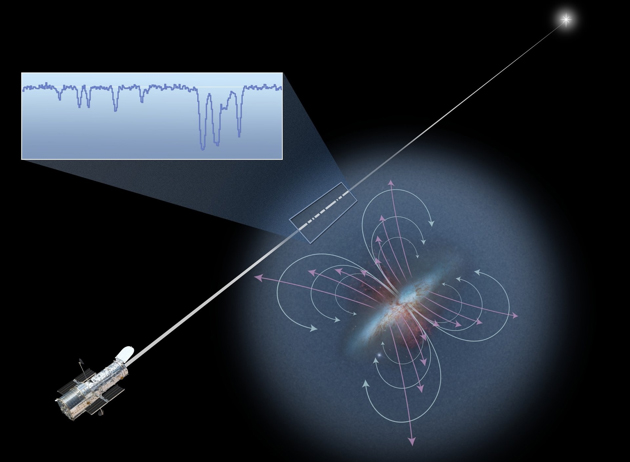
\includegraphics[width=0.45\textwidth]{hubble_cgm.jpg}
  \caption{\small{Artist impression of the Hubble Space Telescope measuring galaxy halo gas absorption in the spectrum of a background QSO (image credit: NASA/STScI/Ann Feild). See below for a real example of measured CGM absorption in a COS spectrum.}}
  \label{hubble_cgm}
  \vspace{10pt}
  \end{centering}
\end{figure}


\begin{figure}[]
  \begin{centering}
  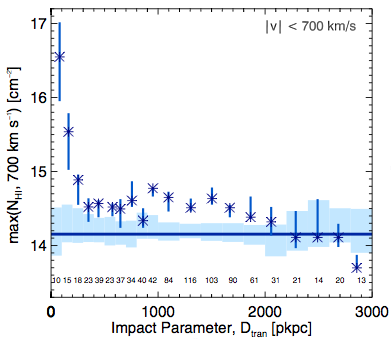
\includegraphics[width=0.45\textwidth]{rudie2012_NvsR.png}
  \caption{\small{Rudie et al. (2012) plot of neutral hydrogen column density, N(H\,{\sc i}) vs impact parameter to the nearest associated galaxy. A clear excess is seen out to physical distances of $\sim2$Mpc.}}
  \label{rudie2012}
  \vspace{10pt}
  \end{centering}
\end{figure}


\vspace{15pt}

\section{Scientific Questions}

%\section{Summary of Current Questions:}

\indent There are numerous open questions concerning the interactions of galaxies and IGM absorbers. I propose to address the following four with my Ph.D. thesis:
\vspace{10pt}


\indent \textbullet $ $ \textit{Do the physical properties of absorbers depend on their location and orientation with respect to galaxies?} Recent results suggest that absorbing systems have a preferred orientation with respect to the major and minor axes of the galaxies they are associated with (e.g. Kacprzak et al. 2011, 2012). This could be evidence of inflows and outflows, or an effect of the global structure of galaxy halos, but the statistics are not yet good enough to provide consistent answers. Initial results from our pilot study (described below) suggest a preference for detecting absorbers near highly inclined galaxies (inclination $>50^{\circ}$), and show an intriguing dichotomy between red vs blue shifted absorbers with respect to the systemic galaxy velocity, possibly revealing evidence of inflows (see Figure \ref{dichotomy}; French et al. 2015, in prep). A larger-scale study of inclination and azimuthal angles vs. absorber properties for the largest galaxies in the nearby universe, where it is possible to obtain inclinations and unambiguous absorber associations, is needed in order to elucidate the distribution of absorbing systems around galaxies.

\vspace{10pt}
\indent \textbullet $ $ \textit{How strongly is intergalactic gas concentrated near galaxies, and do galaxies affect the physical conditions of the intergalactic gas?} Recent studies find that half of all Ly$\alpha$ absorbers lie within galaxy halos, at impact parameters $\rho<350$kpc and within 400 km/s of the associated galaxy (C\^{o}t\'{e} et al. 2005, Prochaska et al. 2006, Wakker $\&$ Savage 2009 - hereafter WS09). The properties of the lines also appear to change with impact parameter. It has been known for some time that higher column densities are found closer to galaxies (see WS09 and many references therein). In addition, broad lines (FWHM$>$150 km/s) are only seen at impact parameters smaller than 350 kpc (see Figure \ref{moneyplot}).  This phenomenon was also observed at higher redshift by Prochaska et al. (2011), but it remains unclear which physical process is responsible; increased turbulence, increased temperature, an effect of velocity gradients, or a blending of different cloudlets. Studying this phenomenon as a function of 
\begin{figure}[h!]
  \centering
  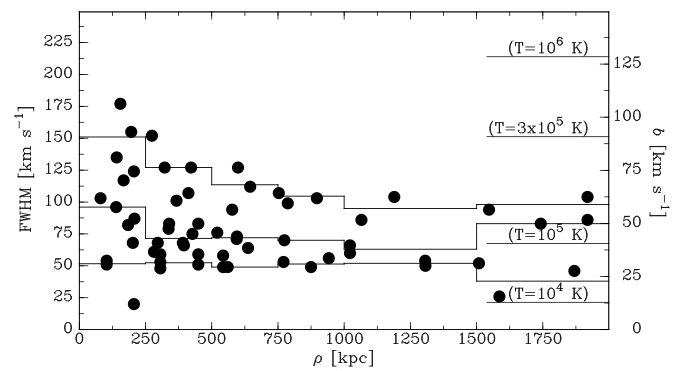
\includegraphics[width=0.51\textwidth]{bart_moneyplot}
  \vspace{-5pt}
  \caption{\small{The width of Ly$\alpha$ lines as a function of impact parameter (WS09). Labels on the right side show the temperatures corresponding to FWHM/b values. The histograms give the 10th, 50th, and 90th percentile of the distribution in 250 kpc or 500 kpc wide bins ($\rho <$ 1 Mpc or $\rho >$ 2 Mpc, respectively).}}
  \vspace{5pt}
  \label{moneyplot}
\end{figure} environment and understanding the properties and morphologies of the nearby galaxies is the clearest way forward on this question. This requires a much larger sample than that used by WS09, which is what our study will achieve. 

\vspace{10pt}
\indent \textbullet $ $ \textit{Does intergalactic gas know about the rotation of the galaxies embedded within it?} In particular, we would like to know how far out (to what impact parameter $\rho$) the rotation curves of galaxies extend. Previous studies (WS09; Kacprzak et al. 2011) were unable to find a clear correlation between $\rho$ and rotation but suffered from a lack of galaxies with known rotation direction. All of these studies are also strongly affected by galaxy sample incompleteness, uncertain galaxy distances, and inconsistent measures of galaxy luminosity. Studying galaxies in the nearby universe makes it possible to obtain orientation information for galaxies, as they can be easily resolved. This aspect of study will benefit especially from the upcoming large ASKAP survey WALLABY (see below), which will map all HI-rich galaxies in the nearby universe, thus allowing us to measure the orientation and rotation direction for any galaxies containing HI.

\vspace{10pt}
\indent \textbullet $ $ \textit{How is the nature of gas within galaxy groups different from that of gas surrounding field galaxies?} WS09 find that for field galaxies a Ly$\alpha$ or Ly$\beta$ absorber can be found in 100$\%$ of cases where a L$>0.1L_{\**}$ galaxy lies within $\rho=350$ kpc of a sightline. For groups this fraction decreases to only $40\%$. This implies that either galaxy groups contain more highly ionized gas than that surrounding field galaxies, or that this gas is more readily swept up due to the higher density of galaxies within groups. However, two major problems with these conclusions remain: (1) group catalogues for nearby galaxies were created over 20 years ago and at that time many galaxies did not have redshifts, so group memberships are liable to change significantly, and (2) the composition and structure of the galaxies within groups has not been considered (e.g. spiral vs elliptical, X-ray properties). A better assessment requires an updated group catalogue and taking into account existing supplementary information for individual galaxies.

\vspace{15pt}


%\begin{figure}[h!]
%\centering
%\begin{subfigure}{.44\textwidth}
%  \centering
%  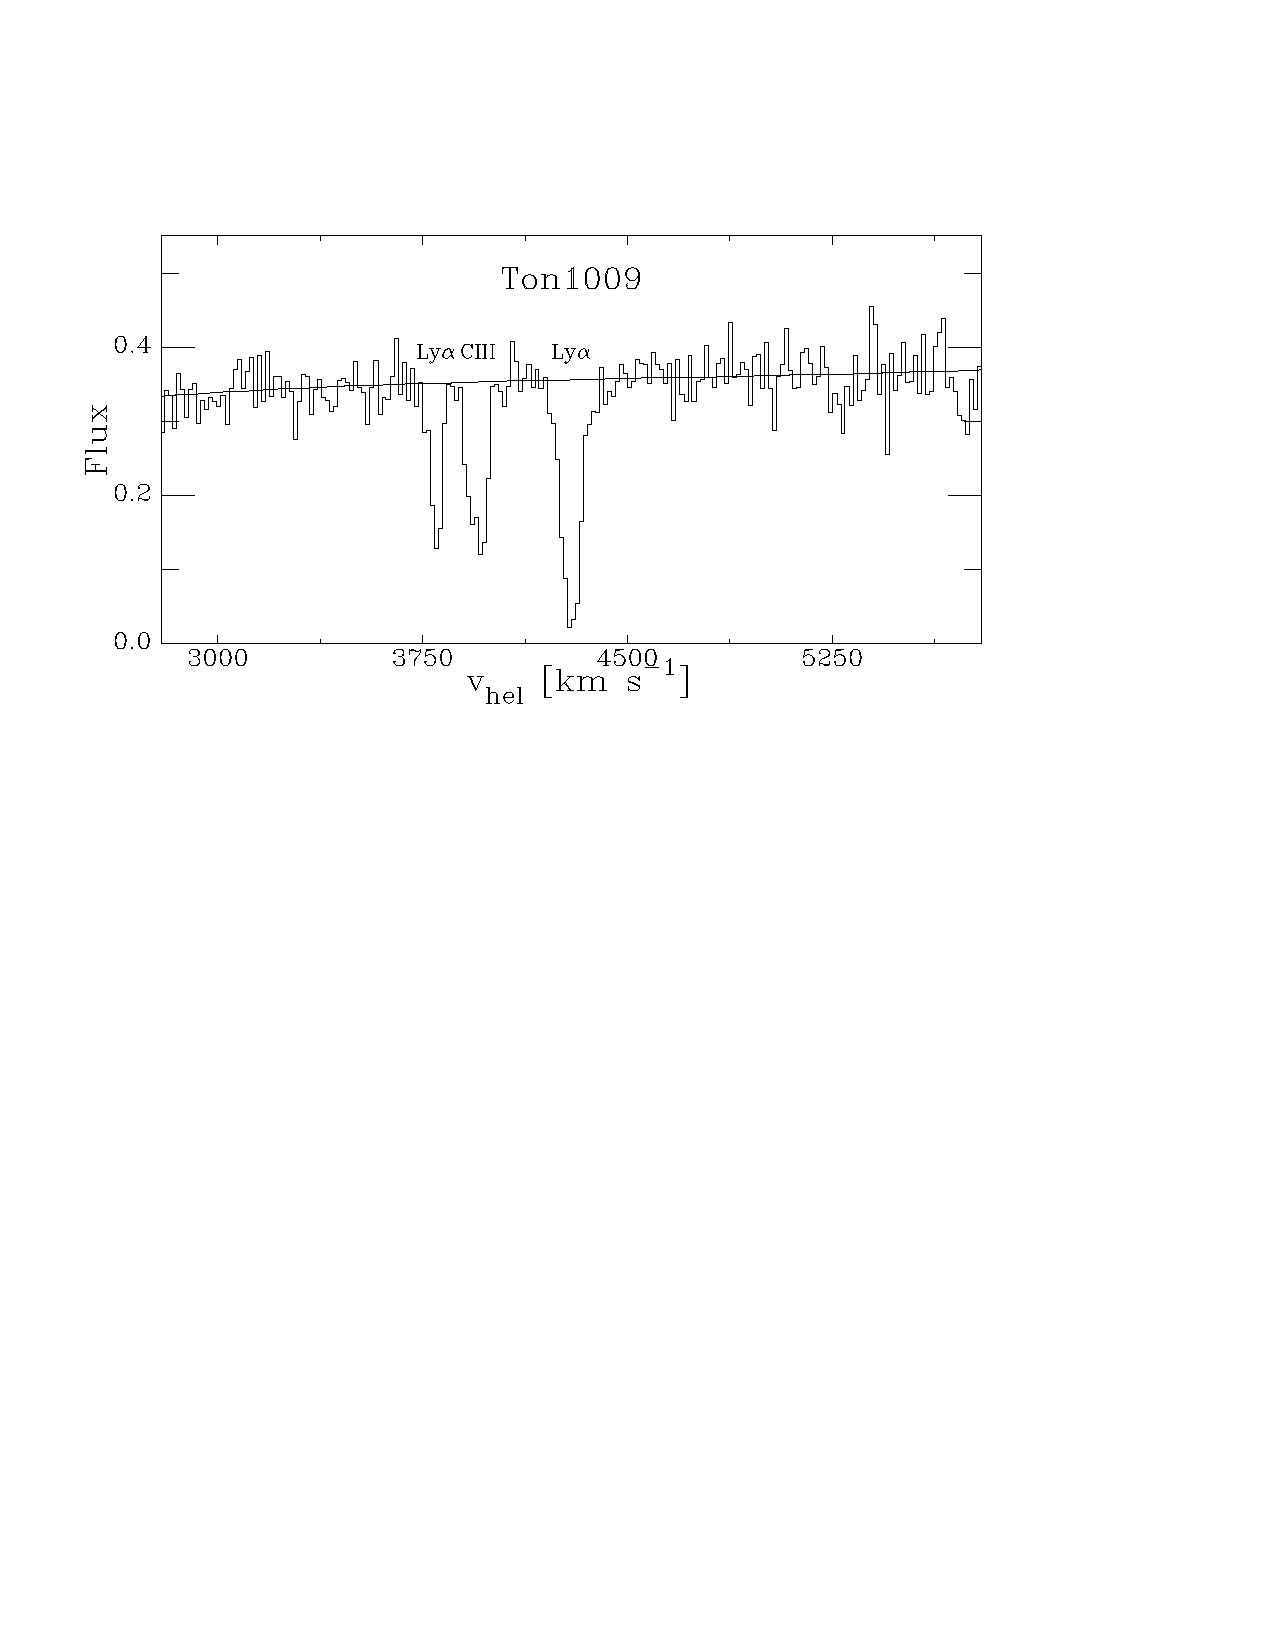
\includegraphics[width=1.0\linewidth]{figTON1009_crop.pdf}
%  \caption{\textbf{ABOVE} An example Ly$\alpha$ line found in a sightline towards target TON1009 at 4295 km/s. (b) \textbf{LEFT} A map of \textit{all} galaxies within a 500 kpc impact parameter target TON1009 sightline and with velocity ($cz$) within 400 km/s of absorption detected at 4295 km/s (central black star). The galaxy IC2439 ($v=4494$ km/s, inclination = $71^{\circ}$) can be unambiguously paired with the Ly$\alpha$ absorption feature at $v=4295$ km/s.}
%  \label{line}
%\end{subfigure}
%\begin{subfigure}{.55\textwidth}
%  \centering
%  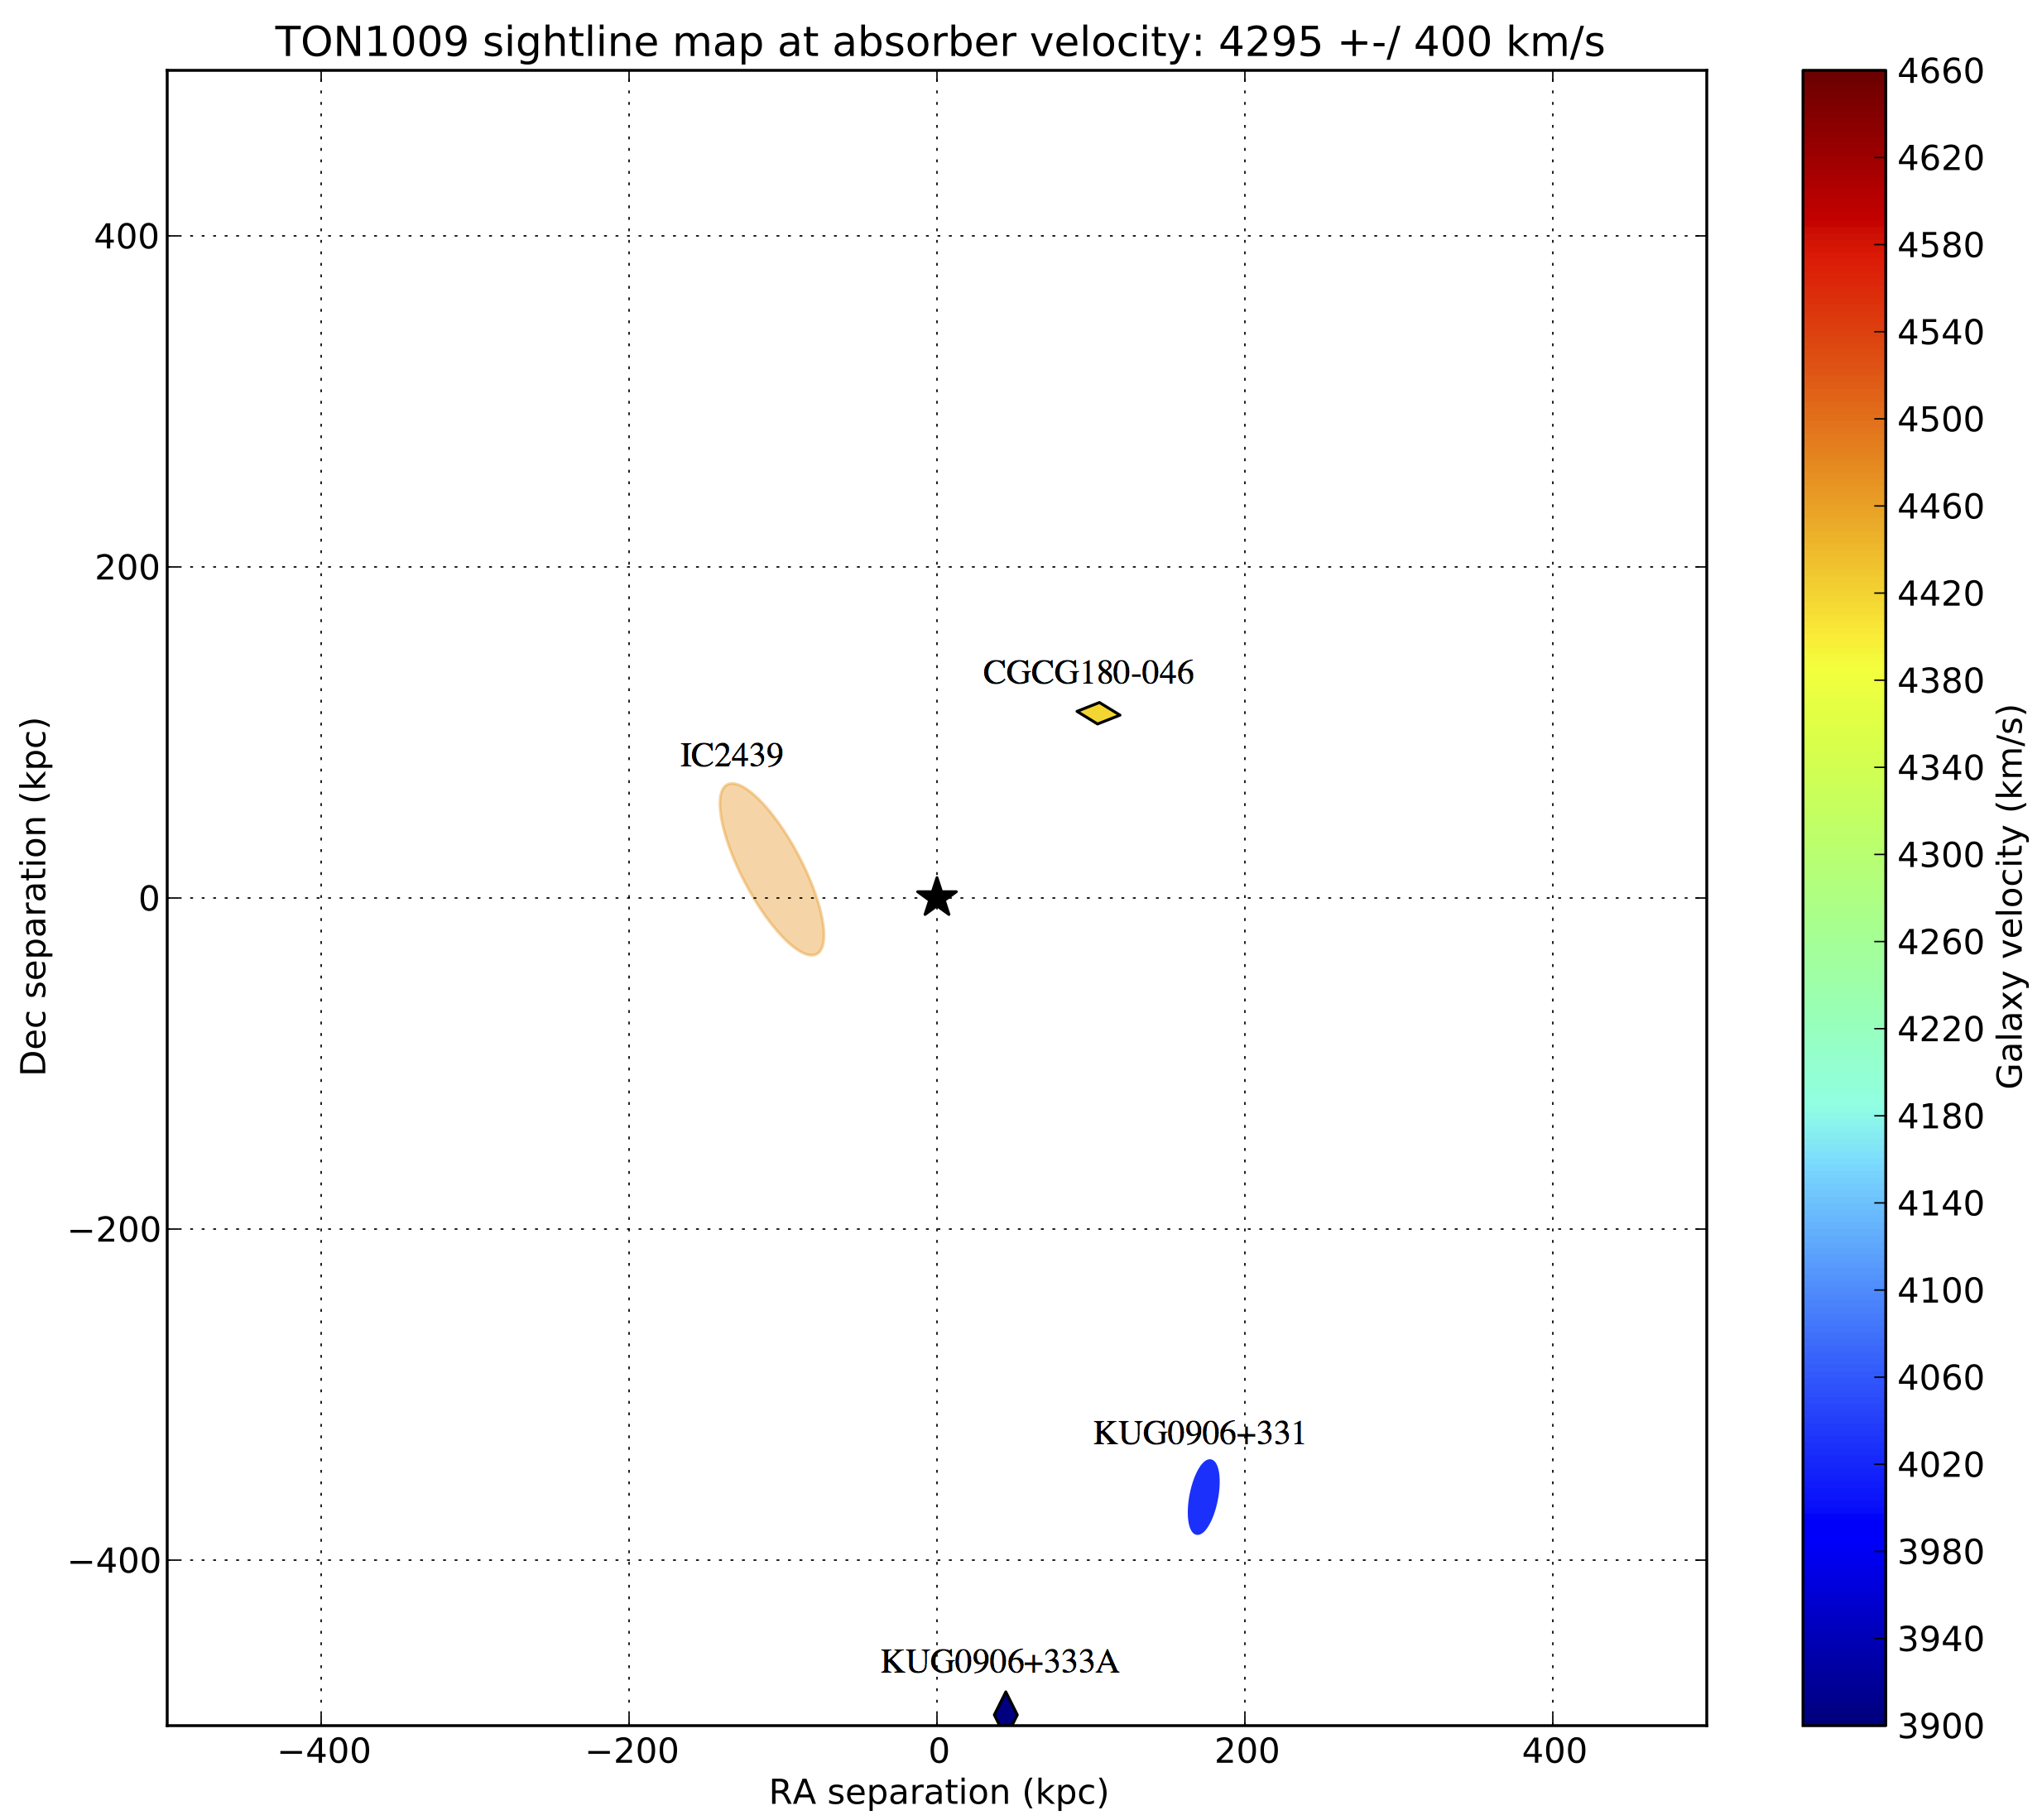
\includegraphics[width=1.0\linewidth]{map2_TON1009_4295_newlabels_crop.png}
%  \caption{}
%  \label{impactmap}
%\end{subfigure}
%\caption{An example Ly$\alpha$ absorption system towards target TON1009. French et al. (2015, in prep)}
%\label{TON1009}
%\end{figure}


\vspace{5pt}
\section{Proposed Program}

\indent To address these questions I will conduct the largest survey to date of intergalactic absorber - galaxy correlations, concentrating on nearby, cz$<$10,000 km/s, systems where the galaxy sample is nearly complete. I will use all UV-bright QSO and Seyfert targets observed with the spectrographs on HST and the Far-Ultraviolet Spectroscopic Explorer (FUSE) to identify all Ly$\alpha$ and OVI absorbers at cz$<$10,000 km/s. Including all new sightlines observed with COS on HST will increase their number from the 76 included in WS09 sample to over 300 (currently), with more to be added dynamically as they are observed over the next 3 years. Whereas previously $\sim100$ absorption systems were found in 76 sight lines out to 5,000 km/s, we expect that going out to 10,000 km/s, combined with the higher S/N spectra produced by COS (allowing us to detected fainter Ly$\alpha$ systems than WS09) will increase our sample size by a factor of 10.  For each target I will identify all detected absorption systems as well as all galaxies with impact parameter $\rho\leq2$ Mpc and velocity 400$\leq$cz$\leq$10,000 km/s. In this velocity range it is possible to get a nearly complete $L\gtrsim0.4L_{\**}$ galaxy sample (complete down to 0.1$L_{\**}$ or better for cz$<2,500$, depending on the region of the sky). 

\subsection{Archival Galaxy Data}
Most CGM studies so far have suffered from the same limitations due to inhomogeneity and incompleteness in the galaxy data. For example, at the average redshift of the sample of Werk et al. 2014, $\langle z \rangle \sim 0.2$, available galaxy data is only complete to $\sim L^{\**}$. Other studies get around this by supplementing the archival galaxy data with new observations, but are then forced to limit their radius of search around the target sightline based on the aperture diameter of the telescope. For example, Mathes et al. 2014 correlate their sight lines with imaging from the WFPC2 camera on HST, but this results in a impact parameter limit of 300 kpc. A galaxy located any farther away from an absorption feature would be completely missed by this approach. As 300 kpc is commonly quoted as the boundary between CGM and IGM gas (based on virial radii and/or escape velocity arguments, e.g. see Stocke et al. 2013 and Mathes et al. 2014), probing gas at and beyond this boundary is essential to developing a full understanding of the galaxy-IGM interface. In order to conduct an unbiased survey of the absorber-galaxy connection, it is necessary to obtain a deep and complete galaxy catalog along each sightline for both detections \textit{and} non-detections of absorbing material.

To create such a sample I have made extensive use of NED to compile a table of all pertinent cz$\leq$10,000 galaxy information. For example, I have collected the redshift, diameter, redshift-independent-distance, morphology, inclination, photometry, and more for each galaxy. NED makes an effort to homogenize these data, but I have gone further by normalizing all measurements of inclination, position angle, size, and luminosity to 2MASS $K$-band values. 2MASS values were chosen for this because it was an all-sky survey, and represents the largest fraction of available galaxy data.
\begin{figure}[h!]
\centering
  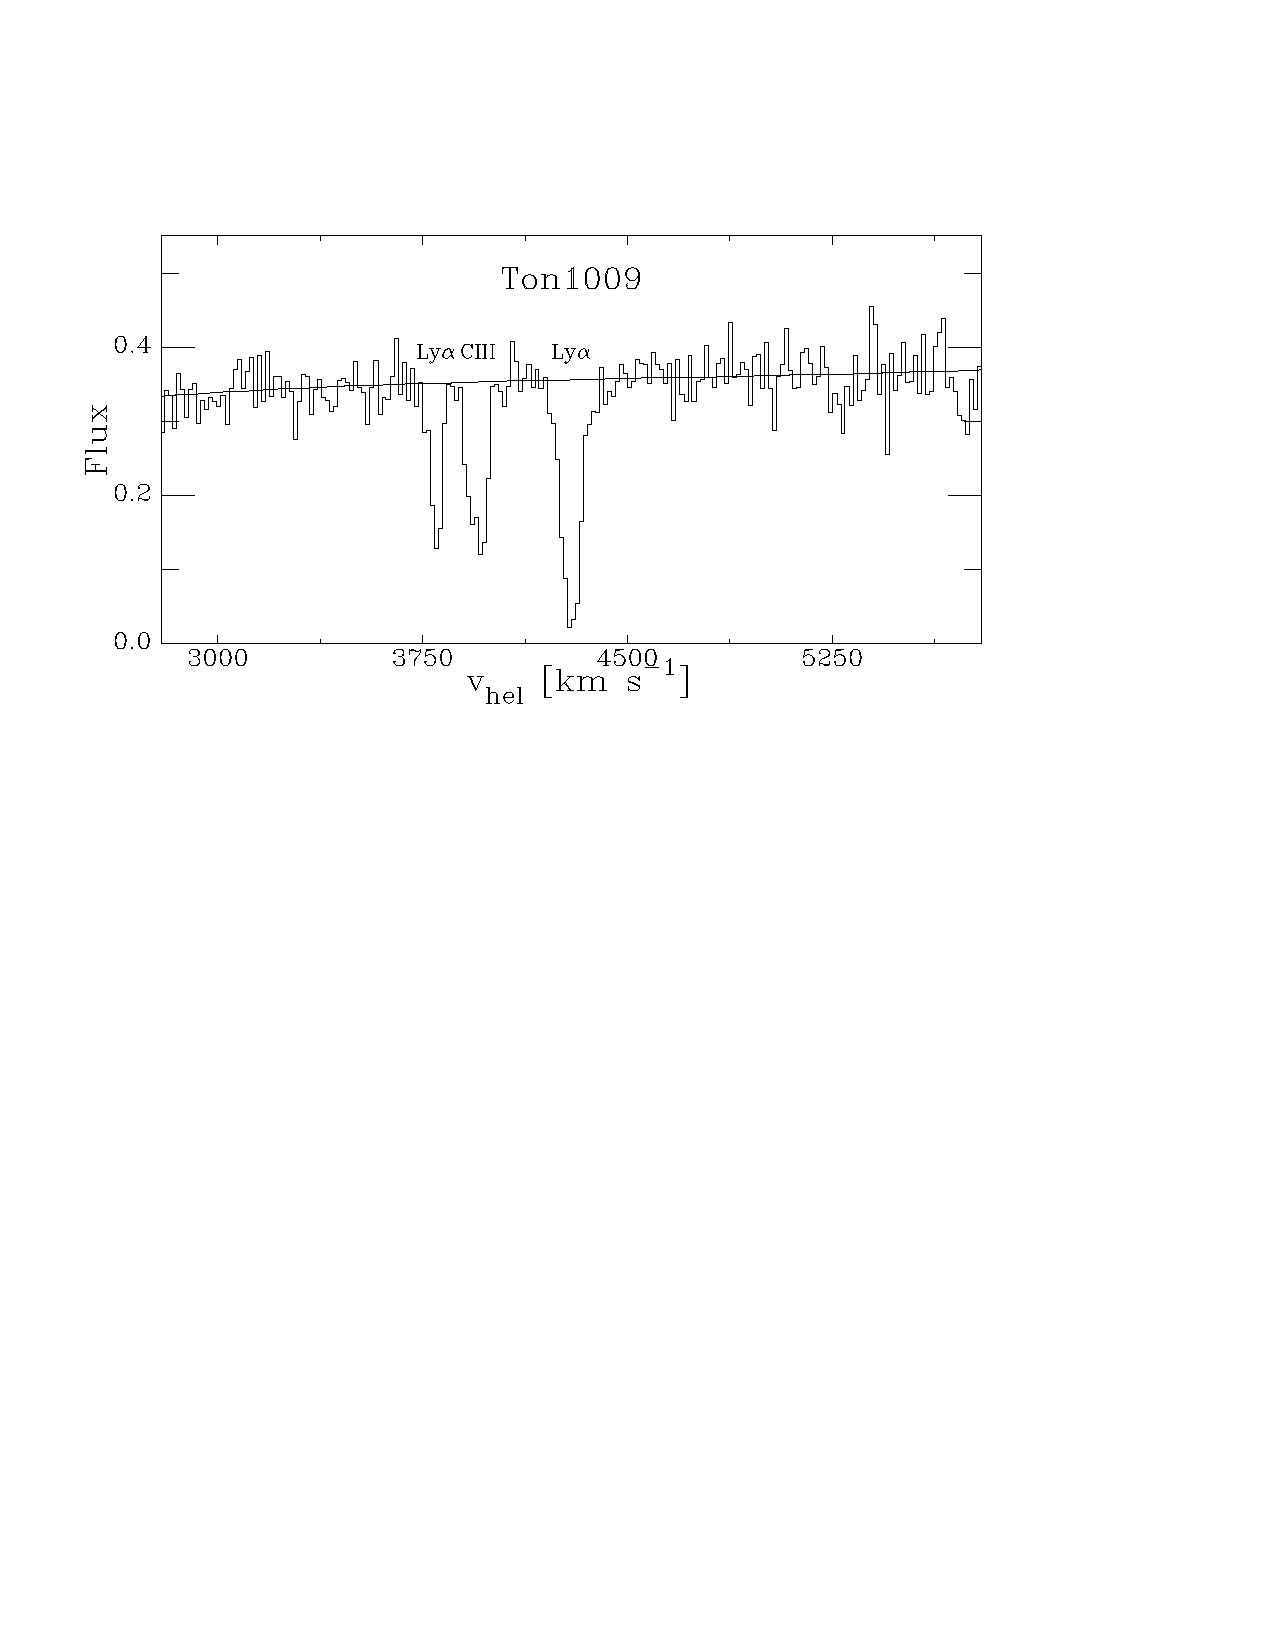
\includegraphics[width=1.\linewidth]{figTON1009_crop.pdf}
  \caption{An example Ly$\alpha$ line found in a sightline towards target TON1009 at 4295 km/s. French et al. (2015, in prep)}
  \label{line}
\end{figure}
\begin{figure}[h!]
  \centering
  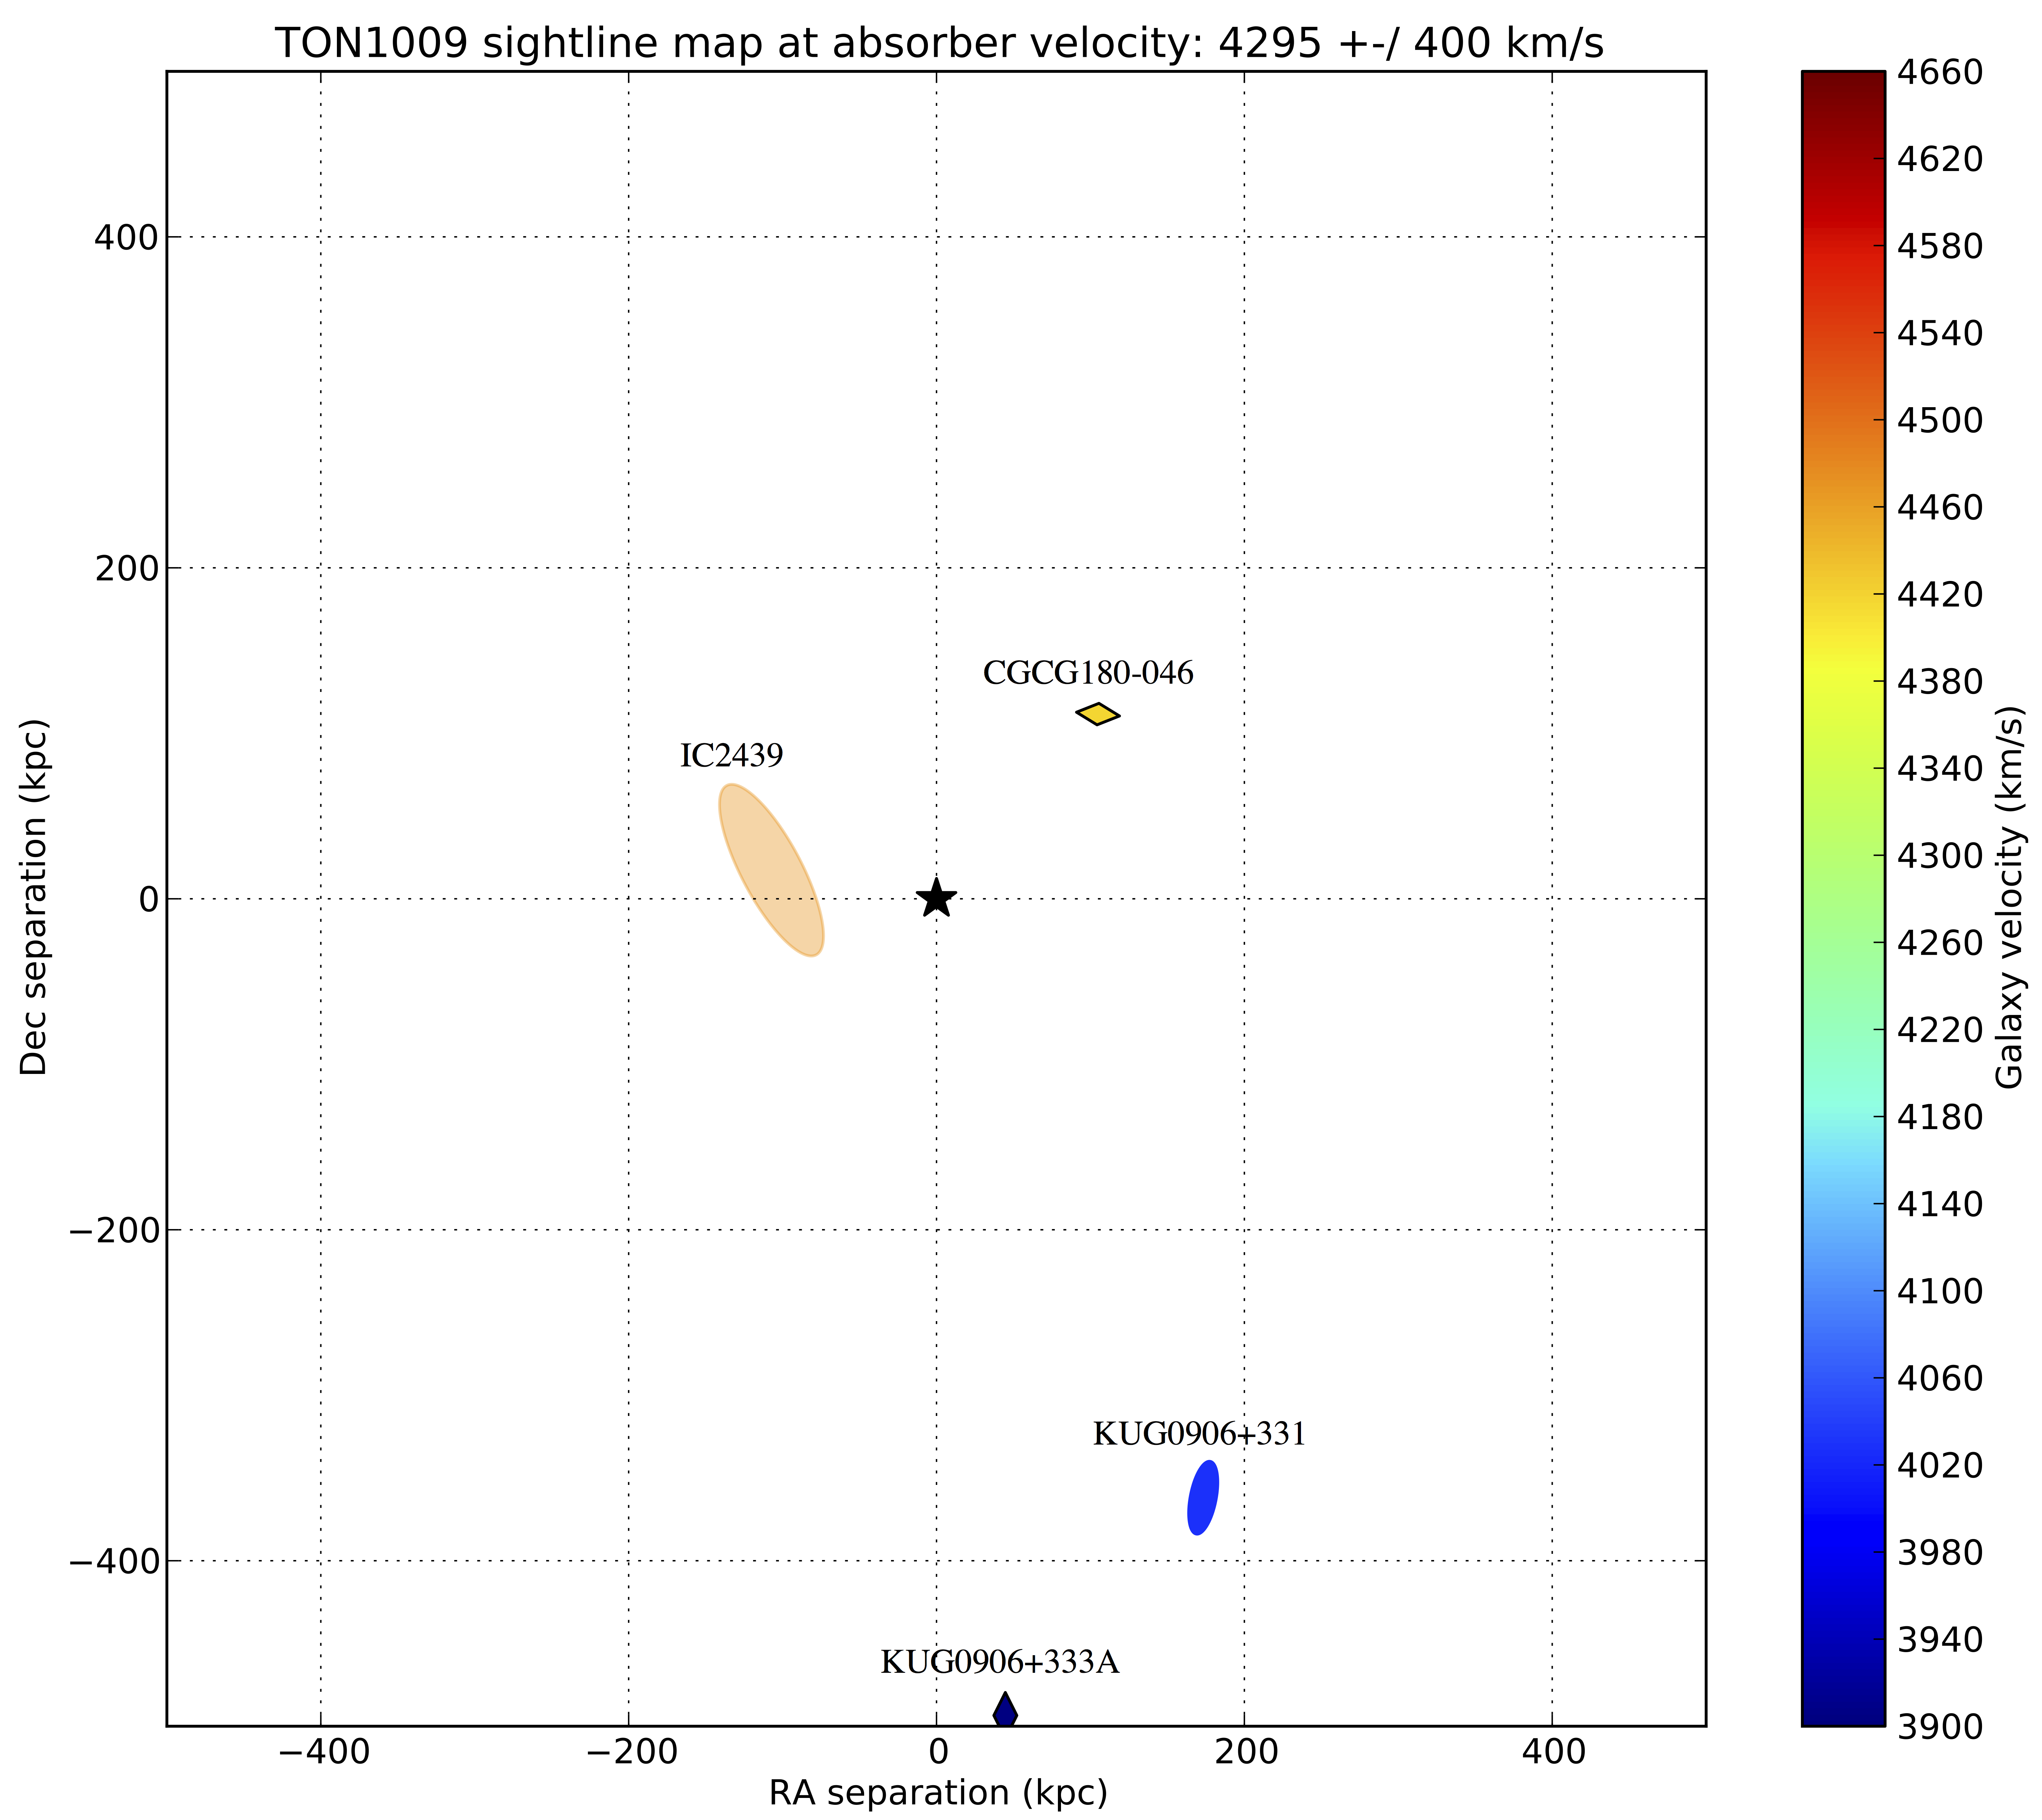
\includegraphics[width=1.\linewidth]{map2_TON1009_4295_newlabels_crop_hires2.png}
  \caption{A map of \textit{all} galaxies within a 500 kpc impact parameter target TON1009 sightline and with velocity ($cz$) within 400 km/s of absorption detected at 4295 km/s (central black star). The galaxy IC2439 ($v=4494$ km/s, inclination = $71^{\circ}$) can be unambiguously paired with the Ly$\alpha$ absorption feature at $v=4295$ km/s because it is the largest and closest galaxy in both physical and velocity space to the absorption feature. French et al. (2015, in prep)}
  \label{impactmap}
\label{TON1009}
\vspace{5pt}
\end{figure} This homogeneous galaxy data table will allow me to draw direct comparisons between the properties of the absorbers and the properties, separations, and environments of nearby galaxies, with unprecedented completeness.


\subsection{Additional Galaxy Observations}

\indent The NASA resources available to me through HST, FUSE, and NED form the essential core of my proposed thesis research. However, the galaxy data available through NED have differing levels of completeness in different regions of the sky. At $cz<5000$, data are mostly from RC3 (de Vaucouleurs et al. 1994) but detailed information is missing for many galaxies. Regions covered by the Sloan Digital Sky Survey (SDSS) have good information for most galaxies with $cz>5000$, but in other regions of the sky our knowledge is spotty. Thus, when necessary, I will also obtain new data from the WIYN 3.5m and SALT 11m telescopes for interesting cases outside the footprint of galaxy surveys such as the SDSS. The ``One-Degree-Imager" (ODI) will be a very efficient instrument for my purposes. For example, a 19th magnitude galaxy can be easily detected in the R band with an 1800 second exposure. After identifying candidate galaxies, I will use the Hydra multi-object spectrograph on WIYN to measure galaxy velocities and rotation directions. This spectrograph has the ability to obtain spectra with R = 1000, S/N = 30 of 19th magnitude objects in $\sim$2-3 hours. I will be collaborating with Keeney et al., who have conducted a WIYN/Hydra galaxy redshift survey around $\sim$50 COS sight lines (Keeney et al. 2013) and who will provide expertise in measuring galaxy redshifts around our sight lines, following the methods described in McLin et al. (2002). 

With the Robert Stobie Spectrograph (RSS) on the SALT 11m telescope we can obtain R=1000 resolution, S/N=50 spectra of a 19th magnitude object in 1 hour. We therefore will be able to increase the sample size of galaxies with known position angle and rotation direction by a factor of $>$10 through long-slit H$\alpha$ observations. 

Further, I will use data from the ASKAP WALLABY survey, in which Dr. Wakker is a CoI. This survey will map the 21-cm sky at dec $<30^{\circ}$ out to z = 0.2 (cz = 60000 km/s) with 10'' and 4 km/s resolution. This will provide rotation curves for \emph{all} galaxies containing detectable HI. Finally, I will use the NED data and the new observations with WIYN and SALT to build an updated local galaxy group catalogue complete with morphological information.


\subsection{Analysis}
All COS spectra will be obtained from the Multimission Archive at Space Telescope (MAST) archives and the CALCOS pipeline will be used for processing the raw data. Individual exposures are then combined by the method of Wakker et al. (2015, submitted), which corrects the COS wavelength scale by cross-correlating all ISM and IGM lines in each exposure. This method corrects the up to $\pm40$ km/s misalignments produced by CALCOS, and produces a corrected error array (based on Poisson noise, which better matches the measured error). Multiple exposures are combined by adding up the total counts in each pixel and then converting back to flux using the original, average flux-count ratio at each wavelength.

All spectral features in the pilot study sight lines were identified by hand, but this will be inefficient given the full set of $\sim300$. To automate this process, I am collaborating with Britt Lundgren on extending her SDSS line-finding algorithm to accept UV data. The original algorithm was designed to pick out metal absorber doublets in SDSS spectra and then bootstrap its way through the remaining spectral features based on line-strength probabilities (for a full description and examples, see York et al. 2005; Lundgren et al. 2009; D. G. York et al., in preparation). For our purposes here, we are adding the option for the algorithm to instead search by Lyman series, with an updated list of line-strength probabilities. Each completely identified target will then be inspected by eye before proceeding with fitting. Once identified, we will use the VPFIT package (see Carswell et al. 2002, Kim et al. 2007) to fit Voigt profiles to individual absorption lines. 


\section{Pilot Study}

\indent We are now completing an initial study of 35 QSO sightlines chosen for their proximity to large galaxies (impact parameter $\leq$ 500 kpc) and their high S/N (S/N $\ge$ 10). All spectra were obtained from the MAST archives. Multiple exposures were combined by cross-correlating interstellar and intergalactic absorption lines, and aligning the Galactic absorption lines with 21-cm spectra. All spectral features were then identified by hand.

%We identified all spectral features in each spectra by eye and made single Gaussian component fits to each, computing equivalent widths via the standard prescription ($W = \int (1- e^{-\tau_{\lambda}})d\lambda$). 

For each detected Ly$\alpha$ absorption component, we correlate with the galaxy environment to generate impact parameter maps centered at the systemic velocity of the absorption. Figure \ref{TON1009} shows an example map and Ly$\alpha$ line, where we can clearly see that the galaxy IC2439 is unambiguously associated with this particular Ly$\alpha$ line. By building up a dataset of such unambiguous pairings, we can correlate the absorption directly with the properties of the galaxies.

\vspace{10pt}
\subsection{Summary of Pilot Results}

\indent Our initial sample of 35 sightlines yields 154 Ly$\alpha$ systems, $32\%$ of which can be paired unambiguously with a single galaxy, while $51\%$ reside in relative voids. In agreement with WS09, we find a steep increase in $W$ with decreasing impact parameter, \textit{but only when normalizing for galaxy size}, implying a mass -- baryonic halo scaling relation. Absorbers were also preferentially detected around highly inclined galaxies, with $73\%$ associated with a galaxy of inclination $>50^{\circ}$. We detect only a slight preference for absorption along the galaxies' major axis, with a median azimuthal angle of $39^{\circ}$. Most interestingly, we discovered a dichotomy between absorption redshifted vs blue shifted with respect to the systemic galaxy velocity (see Figure \ref{dichotomy}). This difference is significant, with $\overline{W}$(redshifted) = 192$\pm$10 m\AA, and $\overline{W}$(blueshifted) = 366$\pm$14 m\AA~(French et al. 2015, in prep). Following the suggestions of recent simulations (e.g. van de Voort et al. 2012), this could be indicative of cold, filamentary inflows, which are expected to be denser, and hot, lower density outflows. So far, we have mostly worked on preparing our data (galaxy properties, spectra, spectral identification, etc), but we are now ready to complete analyzing and preparing a letter with the results.


\begin{figure}[h!]
        \centering
        \vspace{-10pt}
        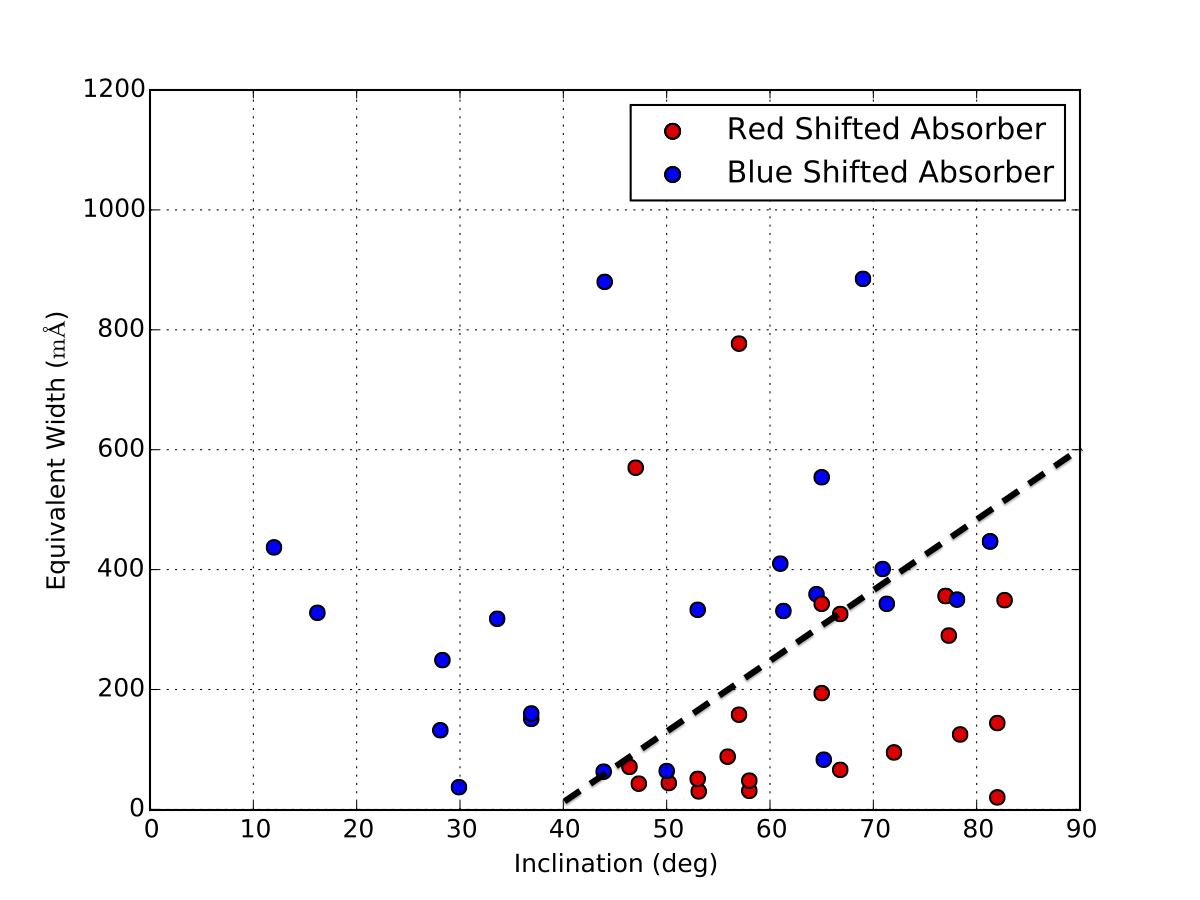
\includegraphics[width=0.52\textwidth]{Wvsinclinationfinal3.jpg}
        \caption{\small{Equivalent width ($W$) of each absorber as a function of the inclination angle of the associated galaxy in the pilot study sample (French et al 2015, in prep). The dashed black line is drawn to highlight the separation between red and blue shifted absorption systems (with respect to the systemic velocity of the galaxy).}}
%        \vspace{-5pt}
        \label{dichotomy}
\end{figure} 




%\begin{SCfigure}[][h!]
%\centering
%\begin{subfigure}{.49\textwidth}
%  \centering
%  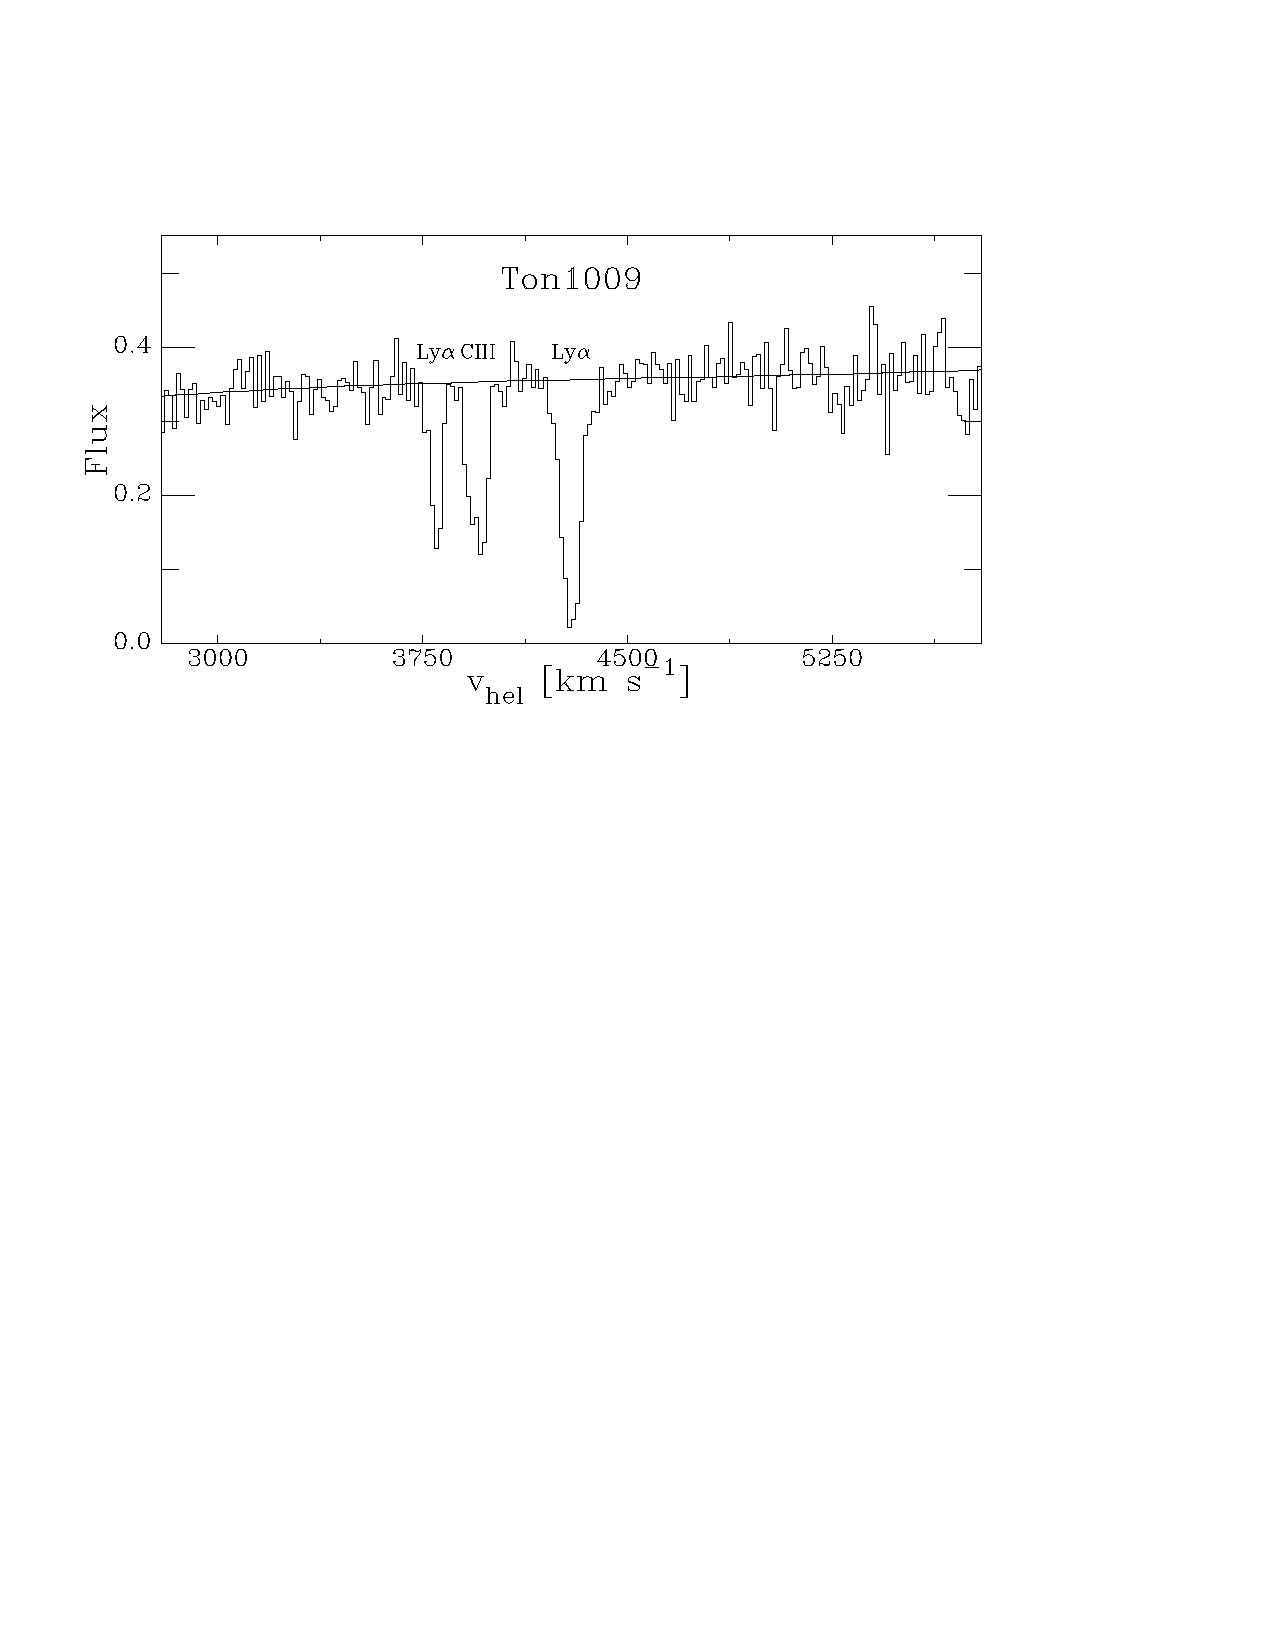
\includegraphics[width=.99\linewidth]{figTON1009_crop.pdf}
%  \caption{An example Ly$\alpha$ line found in a sightline towards target TON1009 at 4295 km/s.}
%  \label{line}
%\end{subfigure}
%
%
%\begin{subfigure}{.50\textwidth}
%  \centering
%  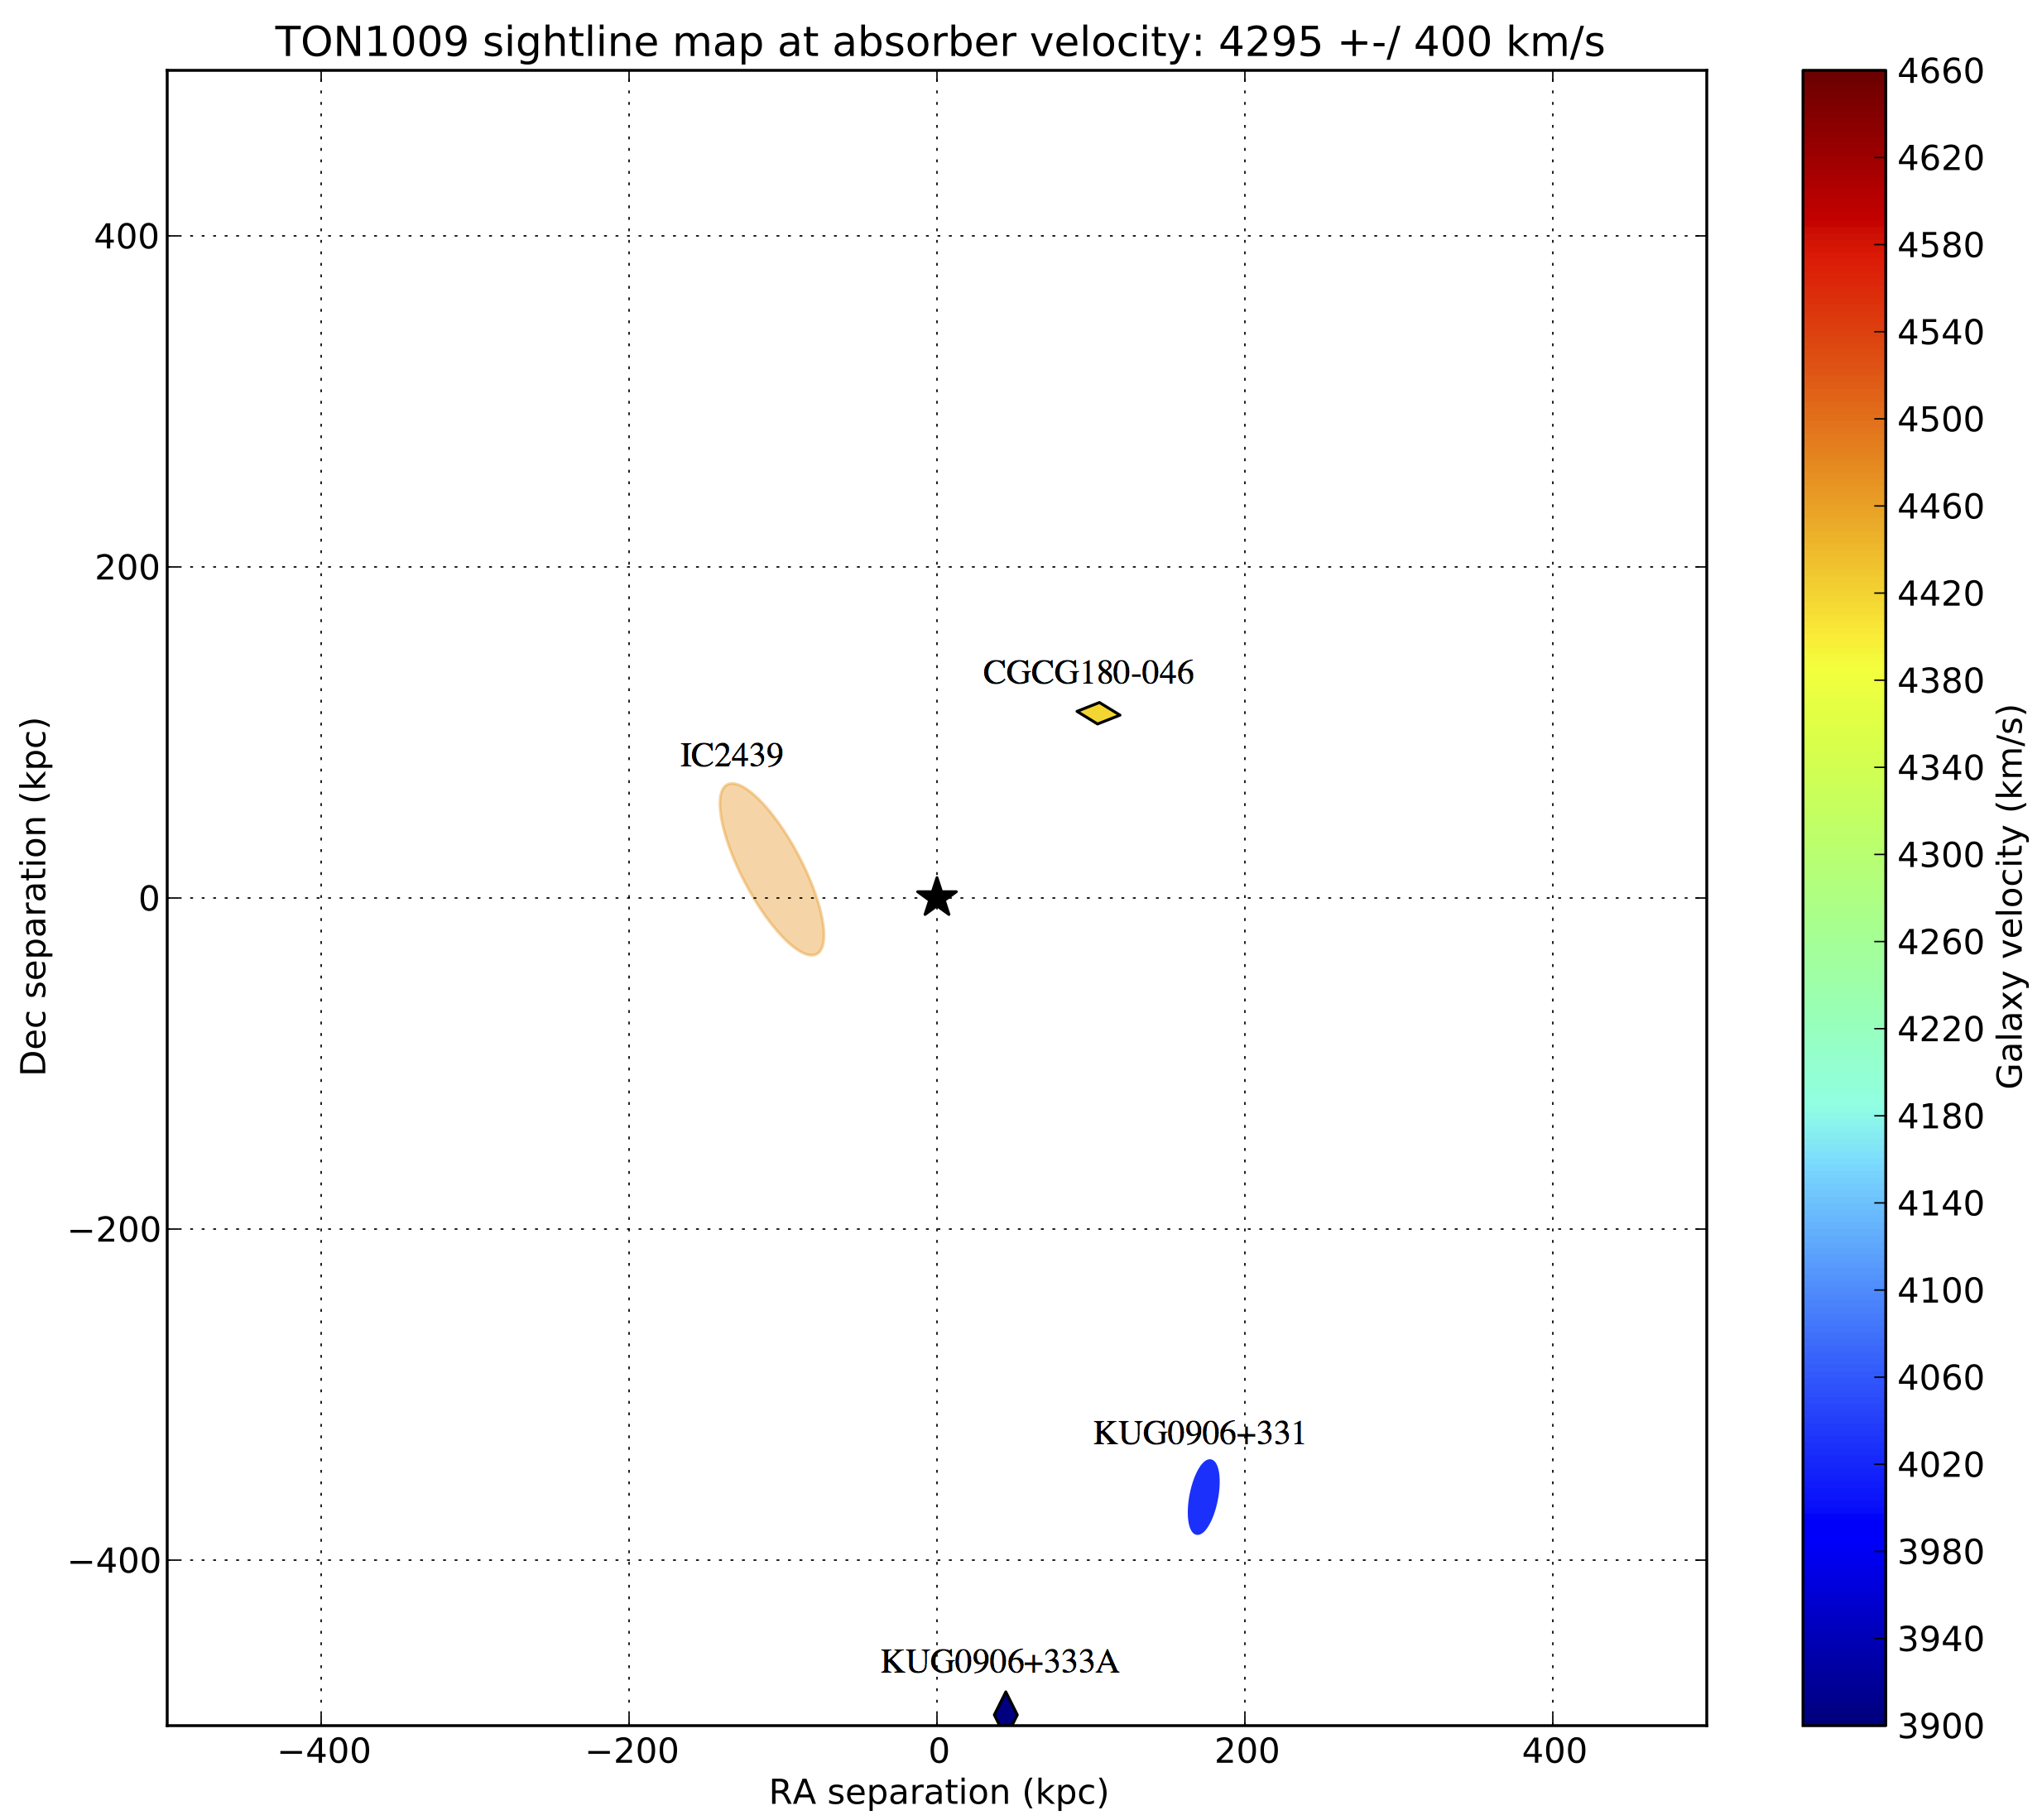
\includegraphics[width=.99\linewidth]{map2_TON1009_4295_newlabels_crop.png}
%  \caption{A map of \textit{all} galaxies within a 500 kpc impact parameter target TON1009 sightline and with velocity ($cz$) within 400 km/s of absorption detected at 4295 km/s (central black star). The galaxy IC2439 ($v=4494$ km/s, inclination = $71^{\circ}$) can be unambiguously paired with the Ly$\alpha$ absorption feature at $v=4295$ km/s.}
%  \label{impactmap}
%\end{subfigure}
%\caption{An example Ly$\alpha$ absorption system towards target TON009.}
%\label{TON1009}
%\end{SCfigure}




%The low redshift (\textit{z}$<$0.5) Ly$\alpha$ forest contains approximately 30$\%$ of the total baryons in the Universe. 
\vspace{10pt}
\section{Comparisons with Simulations}
\indent Much can also be learned about how gas interacts with and is oriented with respect to galaxies by extracting predictions from simulations. $\Lambda$CDM cosmology simulations (e.g. Oppenheimer \& Dav{\'e} 2009; Kere{\v s} \& Hernquist 2009; Smith et al. 2011; Oppenheimer et al. 2012; van de Voort et al. 2012; Cen 2013 \& 2014) concentrate on absorbers originating in galaxy halos (at small $\rho$) or study the Ly$\alpha$ forest statistically (at large $\rho$), but little has yet been done on the intervening region. This region beyond galaxy halos and within 2 Mpc of the galaxies, the region that ultimately provides the source of gas inside galaxies and their halos, is easily resolvable and studied with current simulations, yet few observational constraints currently exist. By extracting individual sight lines from these simulations, we will be able to test the absorption signatures of changing galaxy inclination, size, morphology, and many other properties against real observations. For example, several recent simulations (e.g. van de Voort et al. 2012) suggest blue and red shifted absorption (such as we are seeing in our pilot study; Figure \ref{dichotomy}) could be indicative of cold inflows and hot outflows, respectively. To test this scenario, we will investigate the distribution of metal ion absorption associated with the Ly$\alpha$, as cold, filamentary inflows are expected to be lower metallicity than hot, outflowing gas. The improved statistics from this large data set will ensure reliable results, enabling us to make important strides towards understanding the physical conditions and environments of low redshift absorbers and their relationship with galaxies.

%My proposed work will provide the first large scale observational results constraining this important region of the Ly$\alpha$ forest.

%\begin{figure}
%\centering
%\begin{minipage}{.2\textwidth}
%  \centering
%  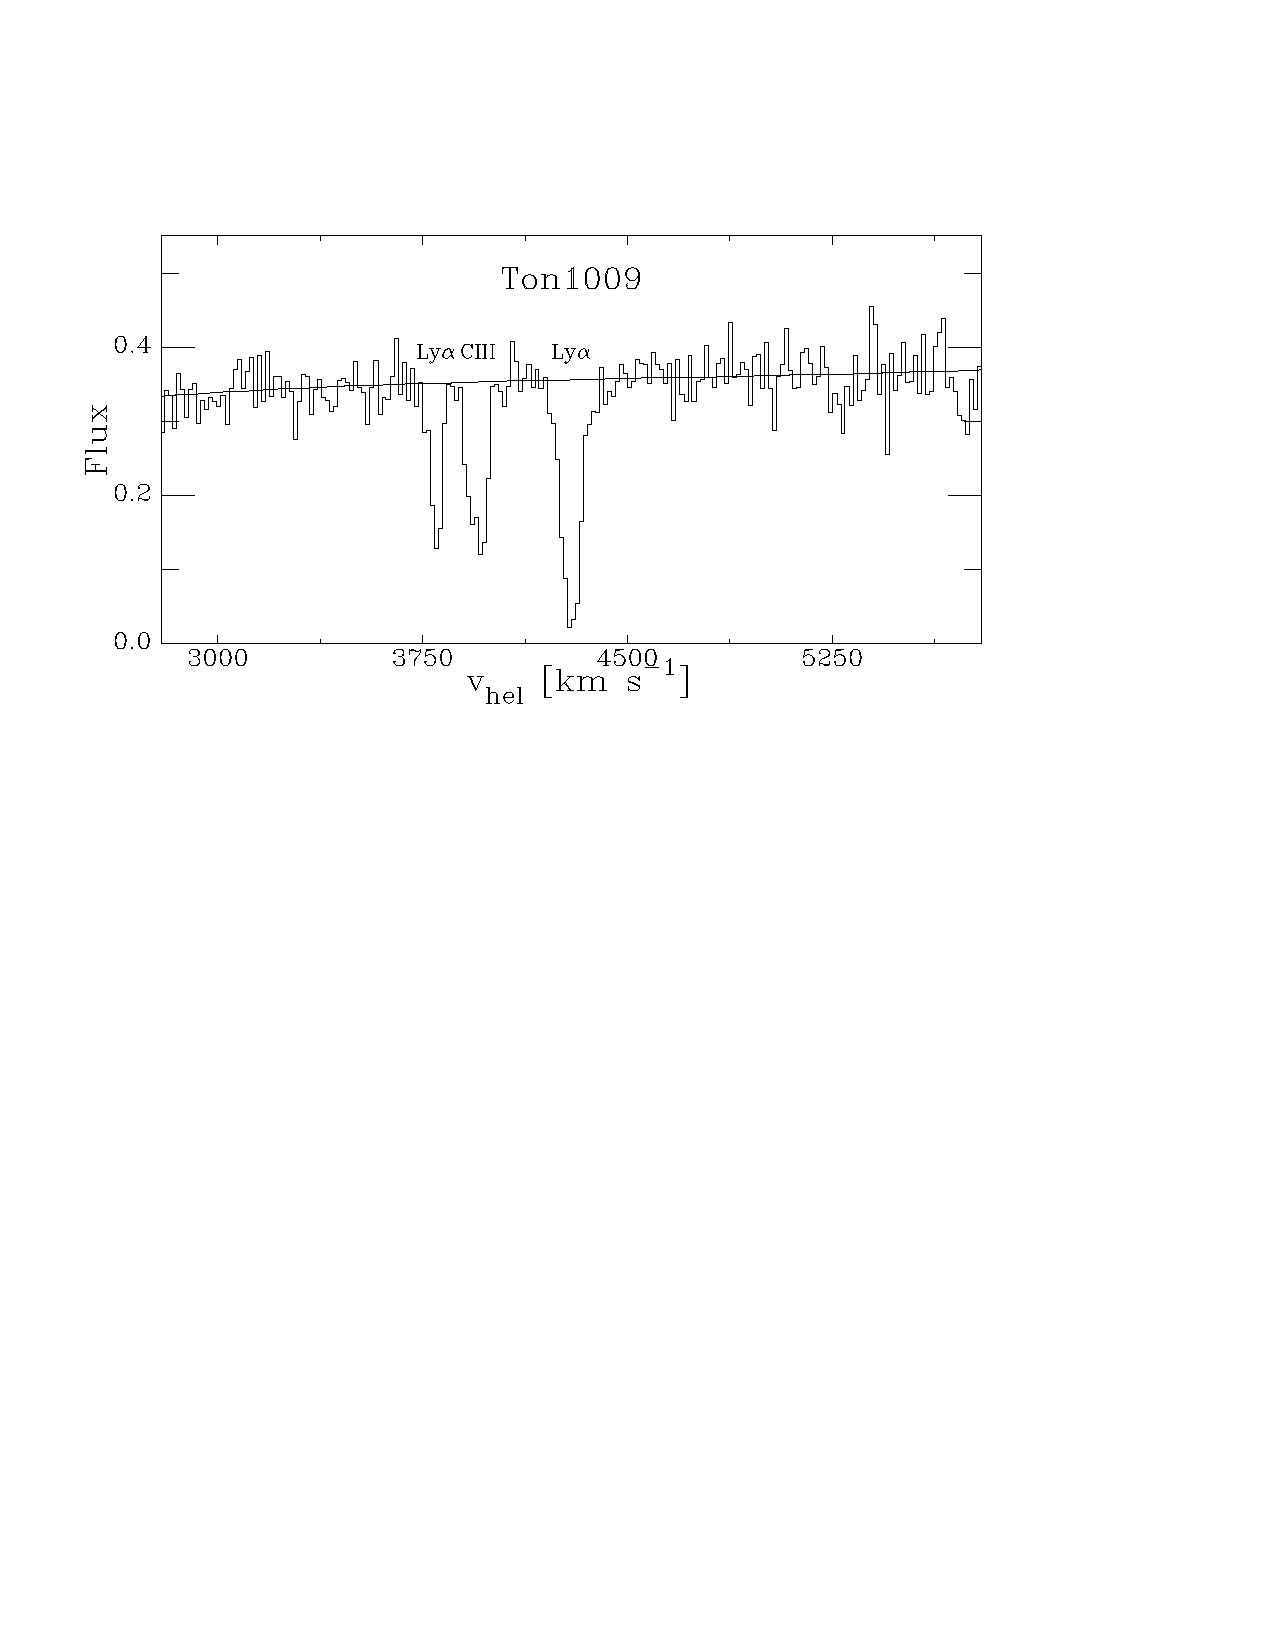
\includegraphics[width=.2\linewidth]{figTON1009_crop.pdf}
%  \captionof{figure}{An example Ly$\alpha$ line found in a sightline towards target TON1009.}
%  \label{line}
%\end{minipage}%
%\begin{minipage}{.2\textwidth}
%  \centering
%  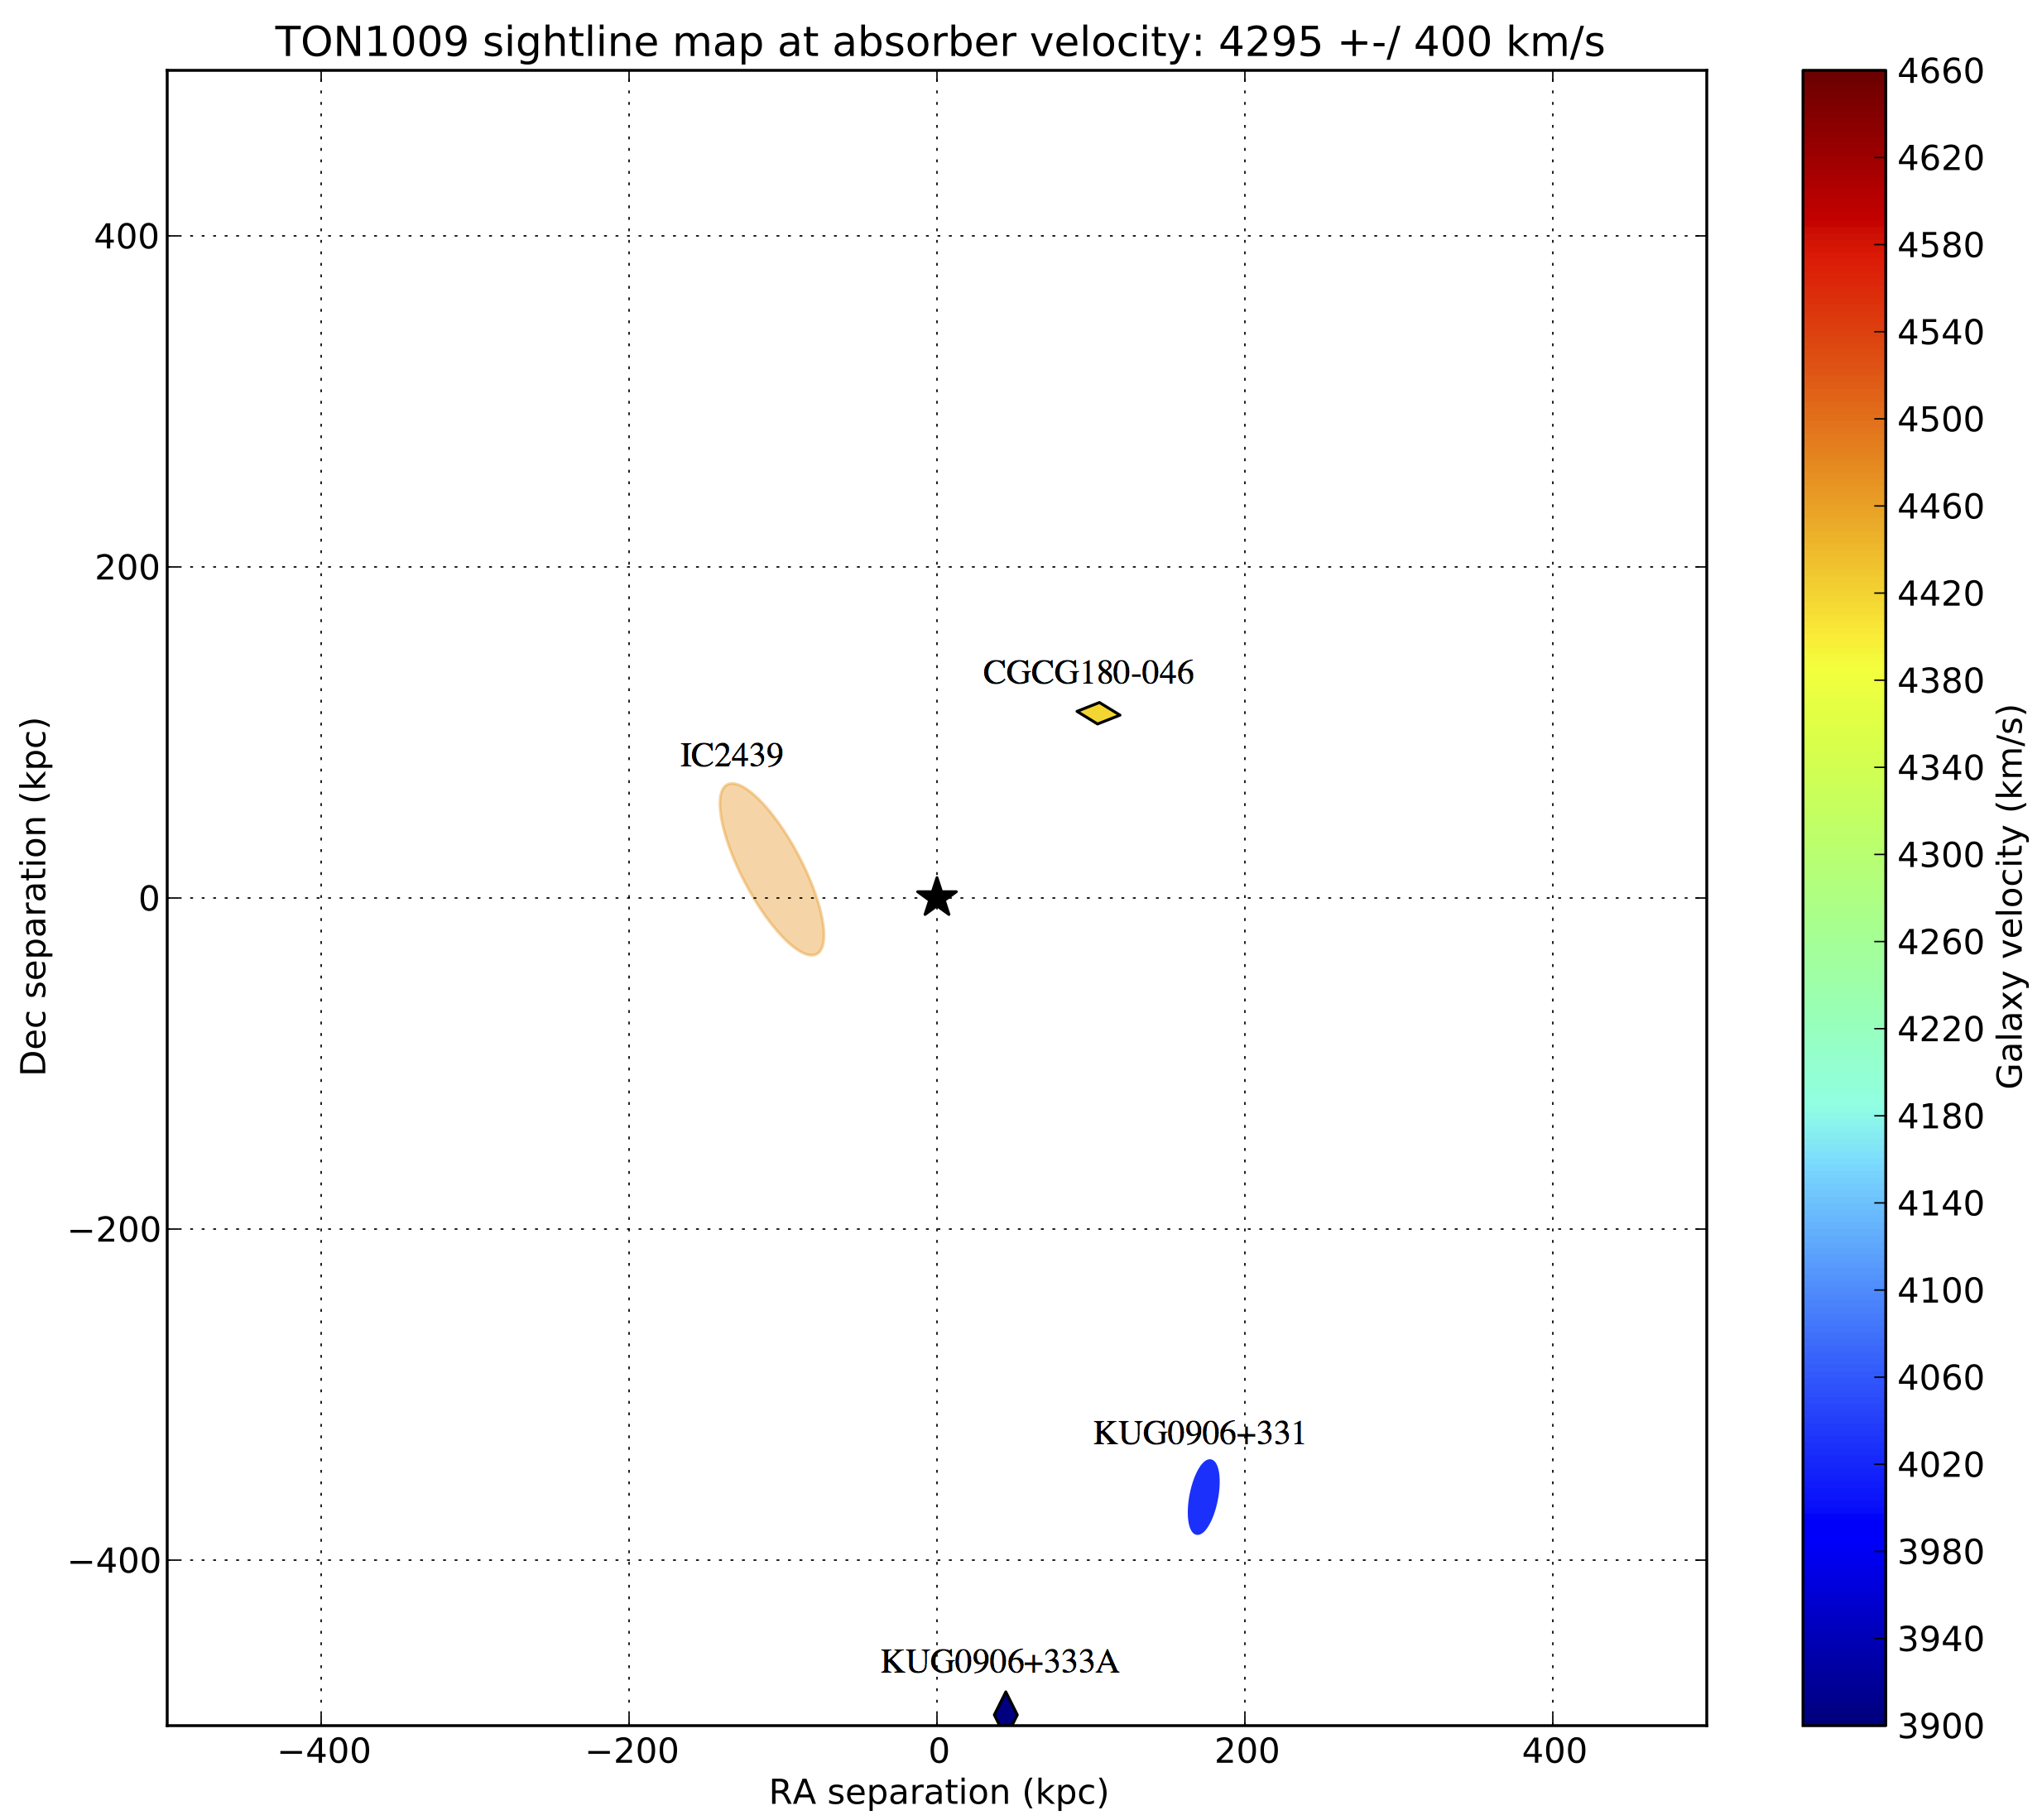
\includegraphics[width=.2\linewidth]{map2_TON1009_4295_newlabels_crop.jpg}
%  \captionof{figure}{A map of \textit{all} galaxies within a 500 kpc impact parameter target TON1009 sightline and with velocity ($cz$) within 400 km/s of absorption detected at 4295 km/s (central black star). The galaxy IC2439 ($v=4494$ km/s, inclination = $71^{\circ}$) can be unambiguously paired with the Ly$\alpha$ absorption feature at $v=4295$ km/s.}
%  \label{impactmap}
%\end{minipage}
%\end{figure}



% \begin{wrapfigure}{r!}{0.61\textwidth}
%        \centering
%        \vspace{-5pt}
%        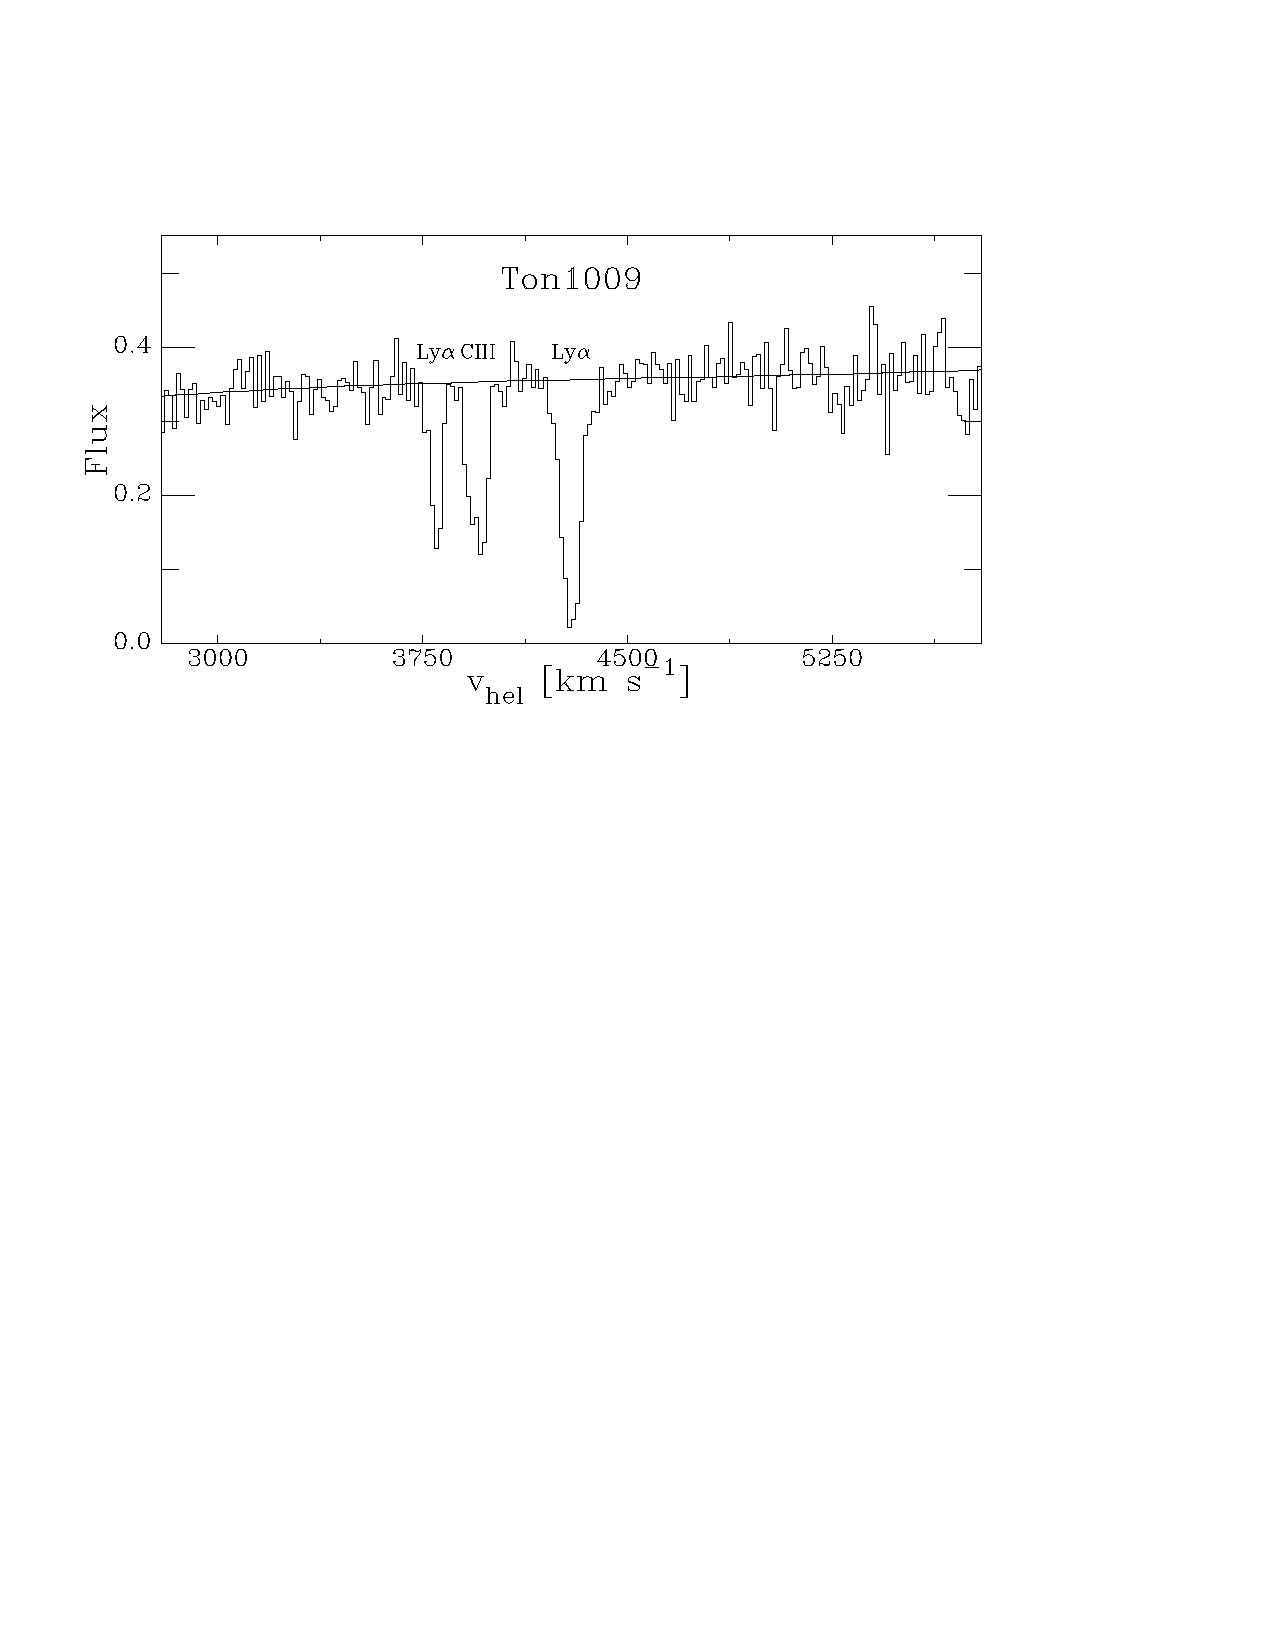
\includegraphics[width=0.62\textwidth]{figTON1009_crop.pdf}
%        \vspace{-20pt}
%        \caption{\small{An example Ly$\alpha$ line found in a sightline towards target TON1009.}}
%        \label{line}
%        \vspace{-10pt}
%\end{wrapfigure}
%
%\begin{wrapfigure}
%  \begin{centering}
%  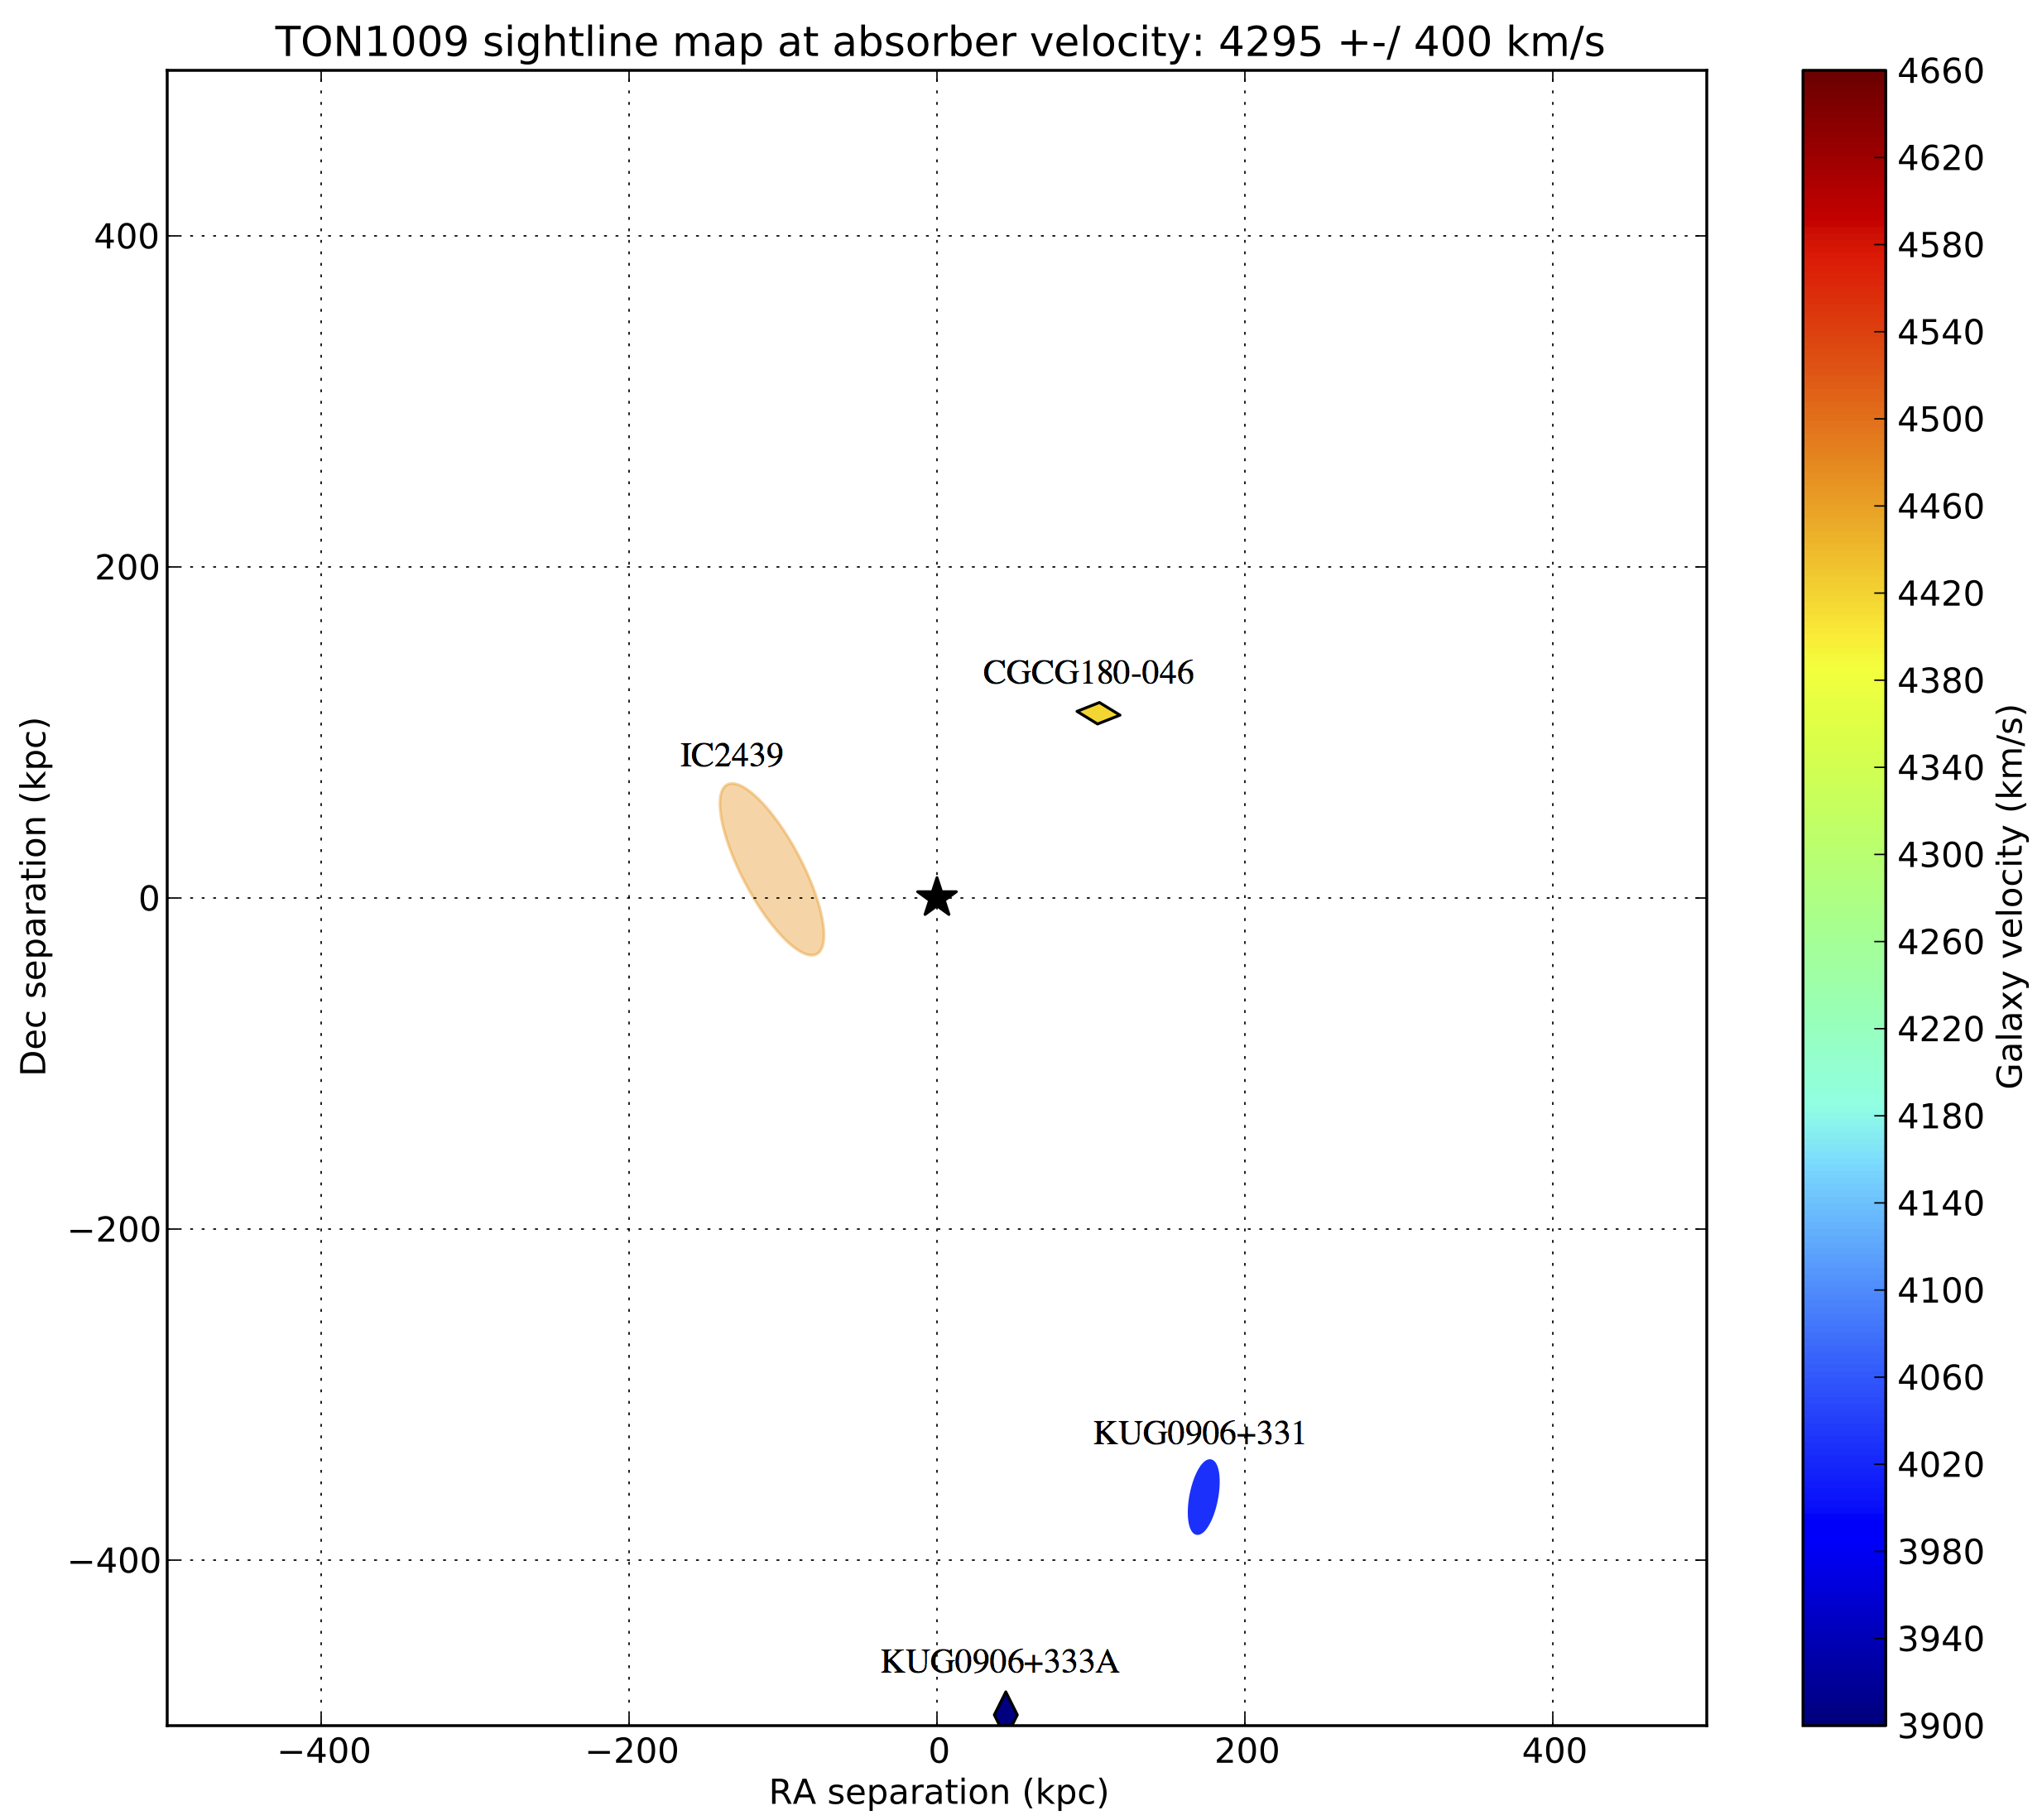
\includegraphics[width=0.99\textwidth]{map2_TON1009_4295_newlabels_crop.jpg}
%  \vspace{-5pt}
%  \caption{\small{A map of \textit{all} galaxies within a 500 kpc impact parameter target TON1009 sightline and with velocity ($cz$) within 400 km/s of absorption detected at 4295 km/s (central black star). The galaxy IC2439 ($v=4494$ km/s, inclination = $71^{\circ}$) can be unambiguously paired with the Ly$\alpha$ absorption feature at $v=4295$ km/s.}}
%  \label{impactmap}
%  \vspace{-5pt}
%  \end{centering}
%\end{figure}

%\begin{figure}[ht!]
%  \begin{centering}
%  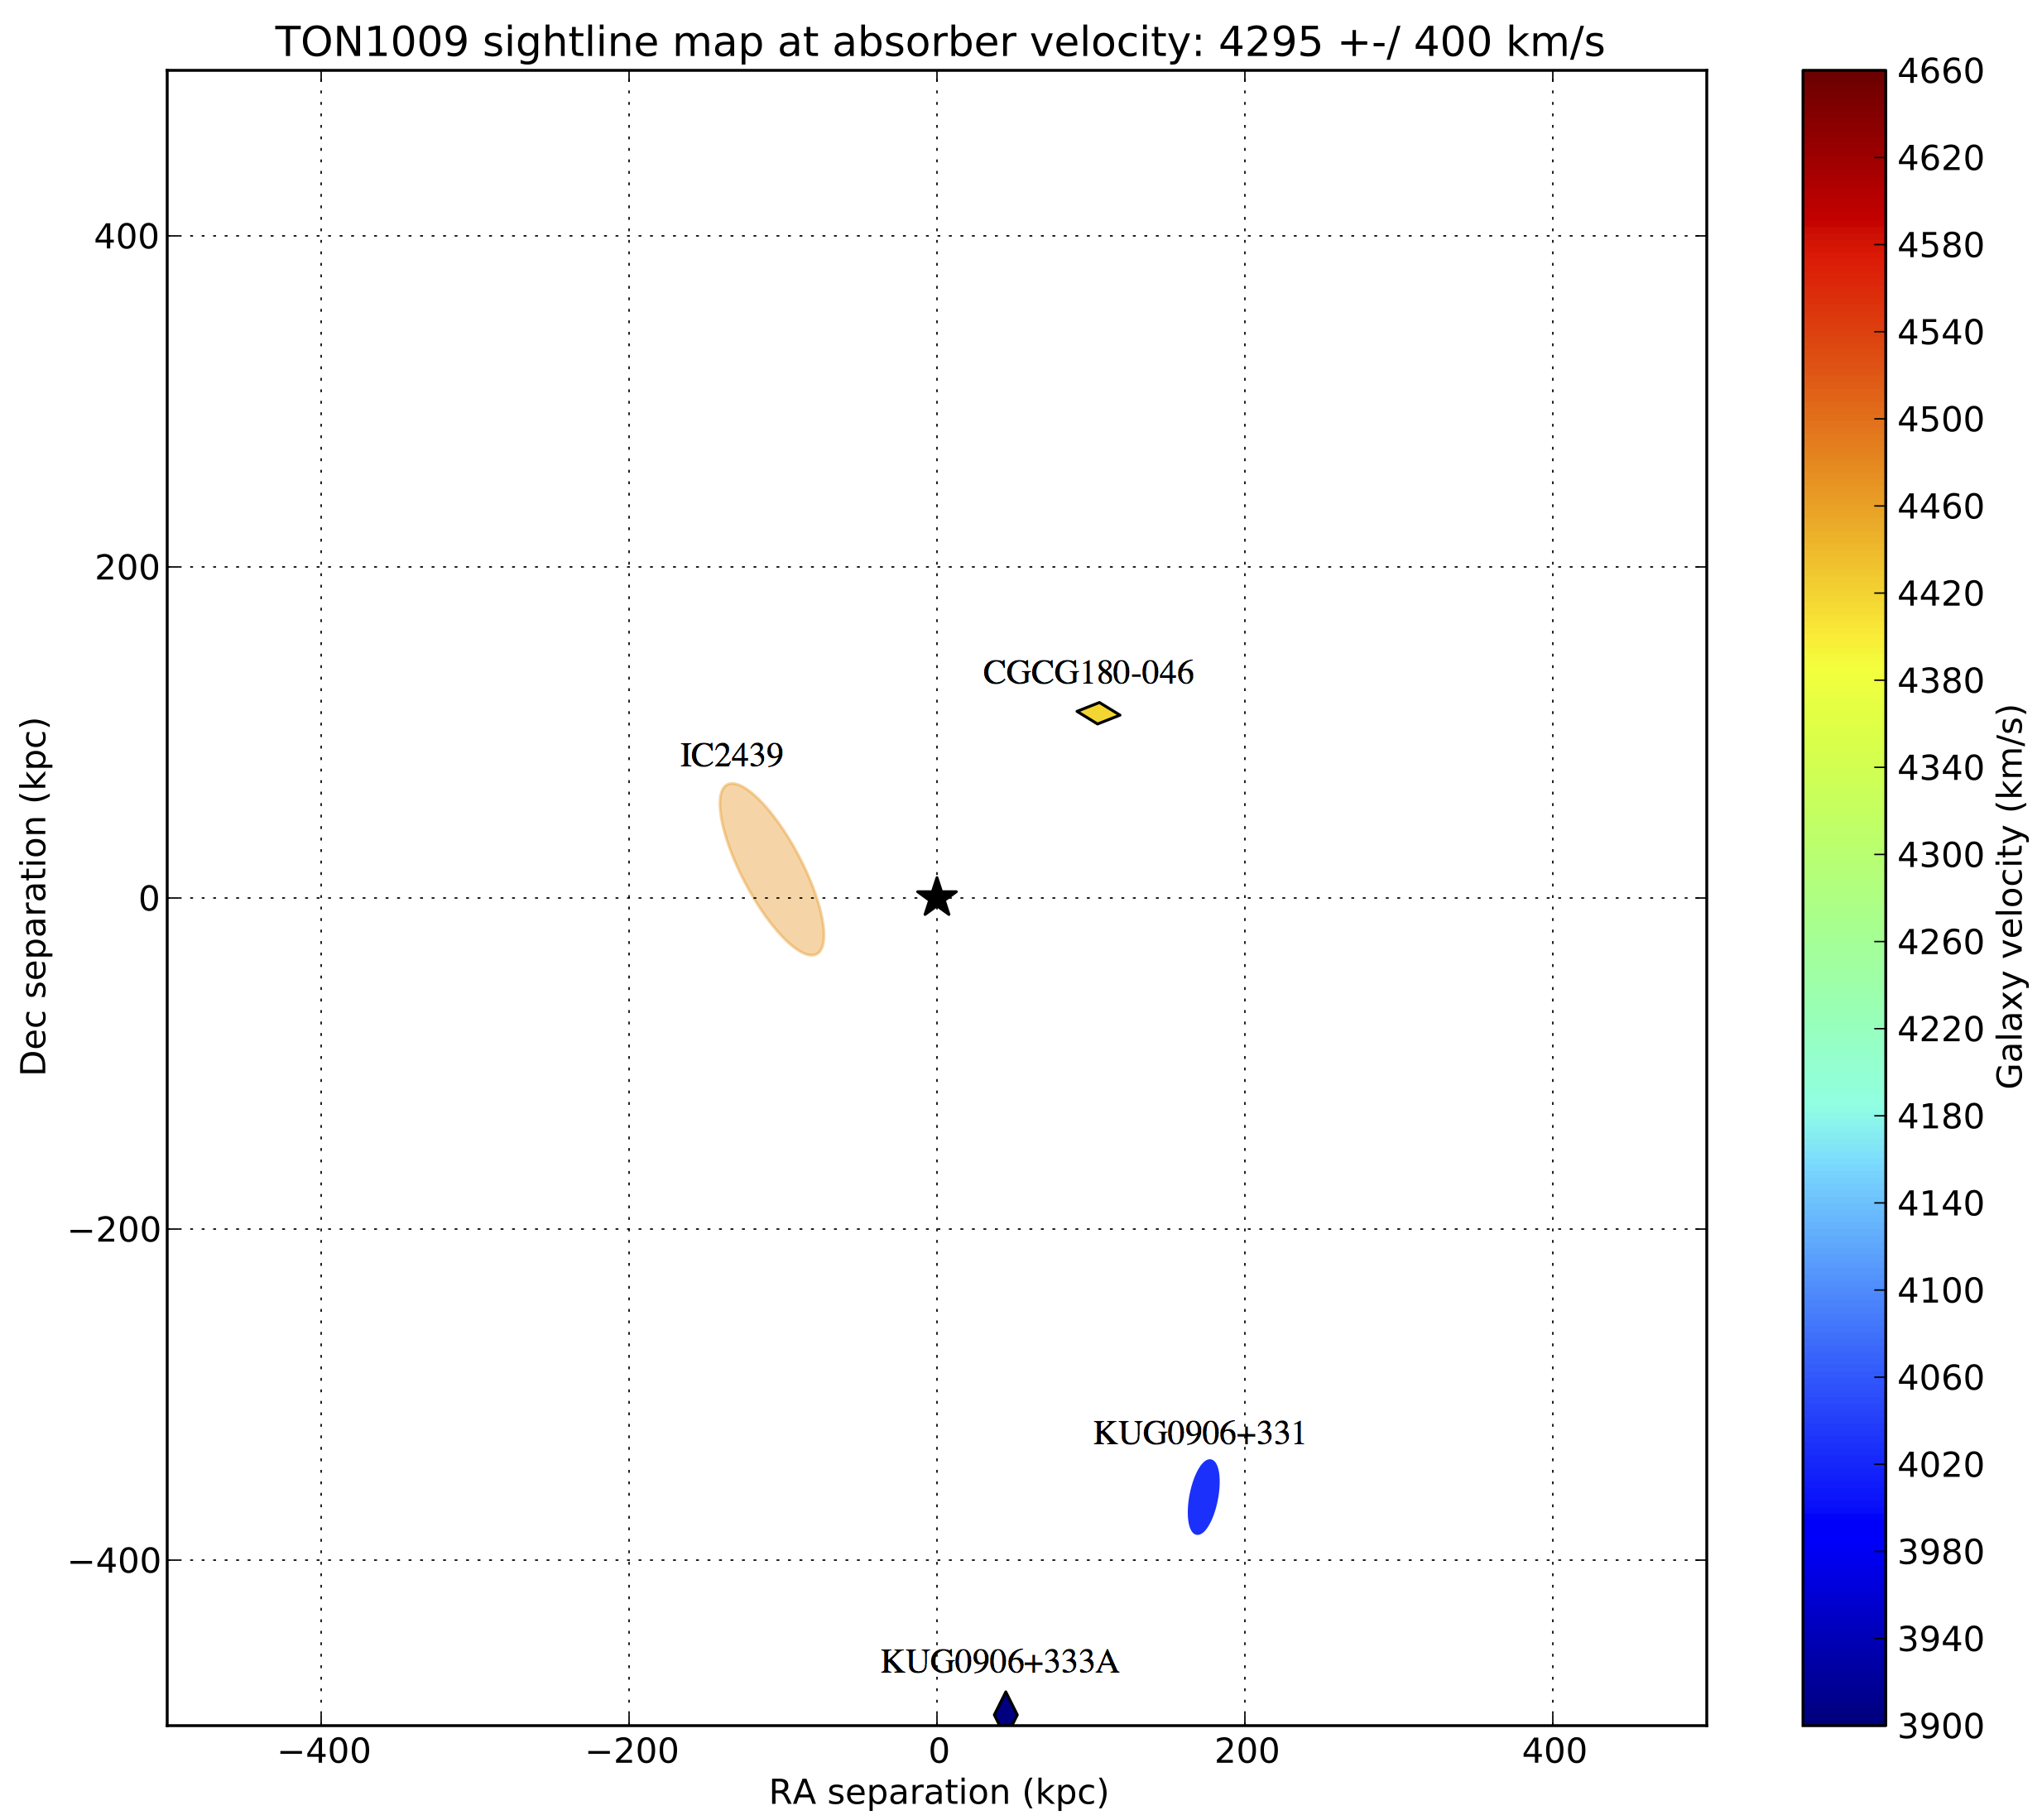
\includegraphics[width=0.99\textwidth]{map2_TON1009_4295_newlabels_crop.jpg}
%  \vspace{-5pt}
%  \caption{\small{A map of \textit{all} galaxies within a 500 kpc impact parameter target TON1009 sightline and with velocity ($cz$) within 400 km/s of absorption detected at 4295 km/s (central black star). The galaxy IC2439 ($v=4494$ km/s, inclination = $71^{\circ}$) can be unambiguously paired with the Ly$\alpha$ absorption feature at $v=4295$ km/s.}}
%  \label{impactmap}
%  \vspace{-5pt}
%  \end{centering}
%\end{figure}


%For example, for each sightline I will construct impact parameter maps such as that seen in Figure 3, which allow me to easily identify the galactic environment associated with each detected absorption. From this I can readily determine that there are two medium sized, nearby galaxies (impact parameter $\rho<1$ Mpc) that have velocities slightly too low ($\sim$6900 km/s), and two large galaxies with appropriate velocities ($\sim$7800 km/s) but slightly higher impact parameter $\rho\sim$1400 km/s. Further investigation of these four possible galaxies may then provide clues to possible interactions with the measured absorbing gas. 
%
%Accurate estimates of galaxy distances will be very important for determining associations between the galaxies and absorbing systems. Redshift distances are particularly suspect in the local universe due to group interactions and local Hubble flows. To obtain better distance estimates, I am using the NED Redshift Independent Distance catalog (NED-D; compiled by Ian Steer, Barry F. Madore, and the NED Team) to supplement the Hubble law derived distances for nearby galaxies. By calculating the peculiar velocities of galaxies as function of position on the sky (using peculiar velocity = $v/H_0 - D$, where $D$ is a NED-D redshift independent distance), I will obtain best-fit Hubble law relations that follow the local Hubble flow. Figure \ref{flow} shows how the best fit Hubble constant varies with velocity to $\sim$10,000 km/s before leveling off (e.g. to $H_0$ = 71 km/s/Mpc used by Wakker $\&$ Savage 2009). This effect was observed by Tully et al. (2013) as well, and demonstrates the need for precise Hubble flow models in order to rely on redshift derived distances. 
%
%\begin{figure}[h!]
%  \centering
%  \vspace{-7pt}
%  \includegraphics[width=0.65\textwidth]{allsky_peculiarVelocities}
%  \vspace{-12pt}
%  \caption{\small{Best fit Hubble constants at peculiar velocity intervals, showing a clear increase in $H_0$ with velocity in the 0 - 10000 km/s range.}}
%  \label{flow}
%\end{figure}



%\vspace{15pt}
%\noindent \textbf{Summary:}\\
%\indent The low redshift (\textit{z}$<$0.5) Ly$\alpha$ forest contains approximately 30$\%$ of the total baryons in the Universe. Much can be learned by studying how this significant reservoir of gas is oriented with respect to and interacting with the galaxies. $\Lambda$CDM cosmology simulations (e.g. Oppenheimer \& Dav{\'e} 2009; Smith et al. 2011; Oppenheimer et al. 2012) either concentrate on absorbers interacting with galaxy halos or study the Ly$\alpha$ forest statistically, but little has yet been done on the intervening region. This region beyond galaxy halos yet within 2 Mpc of the galaxies is easily resolvable and studied with current simulations, yet few observational constraints currently exist. My proposed work will provide the first large scale observational results constraining this important region of the Ly$\alpha$ forest. The improved statistics from this large data set will ensure reliable results, enabling us to make great strides towards understanding the physical conditions and environments of low redshift absorbers and their relationship with galaxies.


%\vspace{15pt}
%\section{NASA Science Mission Directorate:}
%
%\indent My proposed research goals are directly in line with those stated by the NASA Science Mission Directorate (SMD). Using COS observed UV-bright sight lines to understand the gaseous environments surrounding galaxies directly addresses \textsection II.iv of the 2006 NASA SMD Astrophysics Roadmap, \textit{Reveal the Intergalactic Medium}, which states ``Completing the picture will require$\dots$mapping the cooler gas traced by hydrogen absorption and by less highly ionized heavy elements. The Cosmic Origins Spectrograph (COS) would be a valuable step along this path." Understanding how IGM properties correlate with the properties of nearby galaxies is essential for understanding the evolution of the galactic gas supply, and thus the evolution of galaxies. We will make the first large-scale study of the properties of the intergalactic gas in the nearby universe that will be able to address question such as how far galaxy rotation curves extend, whether there is a difference in the properties of the gas surrounding ellipticals and spirals, what differences exist between gas inside and outside galaxy groups, and whether there is evidence for large-scale flows around galaxies.

\vspace{10pt}
\section{Summary}

For my Ph.D. thesis I propose to conduct the largest to date survey of the circumgalactic medium in the nearby Universe. The low redshift (\textit{z}$<$0.5) Ly$\alpha$ forest contains approximately 30$\%$ of the total baryons in the Universe, and much can be learned by studying how this significant reservoir of gas is oriented with respect to and interacting with the galaxies. $\Lambda$CDM cosmology simulations (e.g. Oppenheimer \& Dav{\'e} 2009; Smith et al. 2011; Oppenheimer et al. 2012) either concentrate on absorbers interacting with galaxy halos or study the Ly$\alpha$ forest statistically, but little has yet been done on the intervening region (i.e. the outer CGM, where halo gas merges with the IGM). This region beyond galaxy halos yet within 2 Mpc of the galaxies is easily resolvable and studied with current simulations, yet few observational constraints currently exist. My proposed work will provide the first large-scale, statistically significant, observational results constraining this important region of the Ly$\alpha$ forest. 



\section{Schedule}

\begin{itemize}
\item{Spring/Summer 2015:}
\begin{itemize}
\item PhD Thesis Proposal
\item Finish pilot study analysis of absorption vs inclination angle for large galaxies
\item \textbf{Publish pilot study results}
\end{itemize}

\item{Fall 2015:}
\begin{itemize}
\item Finish reducing and identifying current archived COS sight lines
\item Compile list of galaxies of interest (near Ly$\alpha$ features)
\item Apply for WIYN and SALT time to measure galaxy rotation directions
\end{itemize}

\item{Winter/Spring 2016:}
\begin{itemize}
\item \textbf{Publish full absorption vs inclination angle results}
\end{itemize}

\item{Summer/Fall 2016:}
\begin{itemize}
\item Collect and reduce WIYN and SALT galaxy rotation data
\end{itemize}

\item{Winter/Spring 2017:}
\begin{itemize}
\item \textbf{Publish absorption vs galaxy rotation results}
\item \textbf{Publish line width vs impact parameter results}
\end{itemize}

\item{Summer 2017:}
\begin{itemize}
\item \textbf{Publish final statistical results}
\item Defend and graduate
\end{itemize}

\end{itemize}

%\item{Summer/Fall 2015:}
%\indent \textbullet $ $ Finish reducing and identifying current archived COS sight lines: Fall 2015
%
%\vspace{5pt}
%\indent \textbullet $ $ Apply for WIYN and SALT time to measure galaxy rotation directions: Fall 2015
%
%\vspace{5pt}
%\indent \textbullet $ $ Publish full absorption vs inclination angle results: Fall 2015
%
%\vspace{5pt}
%\indent \textbullet $ $ Begin work on group finding algorithm: Winter 2015
%
%\vspace{5pt}
%\indent \textbullet $ $ Publish updated group catalog: Spring 2016
%
%\vspace{5pt}
%\indent \textbullet $ $ Collect and reduce WIYN and SALT galaxy rotation data: Spring 2016
%
%\vspace{5pt}
%\indent \textbullet $ $ Publish absorption vs galaxy rotation results: Fall 2016
%
%\vspace{5pt}
%\indent \textbullet $ $ Publish line width vs impact parameter results: Winter 2016
%
%\vspace{5pt}
%\indent \textbullet $ $ Defend thesis: Spring 2017
%
%\vspace{5pt}
%\indent \textbullet $ $ Publish final statistical results: Summer 2017
%
%\vspace{5pt}
%\indent \textbullet $ $ \textbf{Expected Graduation: June 2017}\\
%\vspace{15pt}\\


\noindent \textbf{Funding:}
I am supported through Fall 2016 by NSF grant AST-1108913. I have applied for additional funding through the NESSF, and for travel funds from the Wisconsin Space Grant Consortium. I will apply for these next year as well, and will TA one semester if unsuccessful.




%\noindent \large \textbf{References:}

%\vspace{5pt}
%\raggedright
%\small  Cen, R. 2013, ApJ, 770, 139
%
%Cen, R.  2014, ApJL, 789, 21
%
%C{\^o}t{\'e}, S., et al. 2005, ApJ, 618, 178
%
%%Dav{\'e}, R., \& Tripp, T.M.  2001, ApJ, 553, 528 
%
%de Vaucouleurs, G. et al. 1994, AJ, 108, 2128
%
%Kacprzak, G.G., et al. 2011, MNRAS, 416, 3118 
%
%Kacprzak, G.G., et al. 2011, ApJ, 733, 105
%
%Kacprzak, G.G., et al. 2012, ApJL, 760, L7
%
%Keeney, B. et al. 2013, American Astronomical Society Meeting 
%Abstracts, 222, \#214.18 
%
%Kere{\v s}, D. \& Hernquist, L. 2009, ApJL, 700, 1
%
%McLin, K.  et al. 2002, ApJL, 574, L115 
%
%Meiksin, A.A. 2009, RevModPhy, 81, 1405
%
%Oppenheimer, B.D. et al. 2012, MNRAS, 420, 829
%
%Oppenheimer, B.D., \& Dav{\'e}, R.\ 2009, MNRAS, 395, 1875 
%
%Prochaska, J.X. 2006, ApJ, 643, 680
%
%Prochaska, J.X. 2011, ApJ, 740, 91
%
%Rudie, G.C., et al. 2012, ApJ,  750, 67
%
%Shull, J.M., Smith, B.~D., \& Danforth, C.W. 2012, ApJ 759, 23
%
%Smith, B.D. et al. 2011, ApJ, 731, 6 
%
%Tully, R.B. et al. 2013, AJ, 146, 86
%
%van de Voort, F. et al. 2012, MNRAS, 423, 2991
%
%Wakker B.P. \& Savage B.D. 2009, ApJs, 182, 378
%
%\vspace{12pt}

\nocite{*}

\bibliography{paper_bib}
\bibliographystyle{apj}

\end{document}